%% !TeX root = IIII_simulator
% !TeX root = article

% Disallow floats on the first page
\suppressfloats

%Design, notation and application

\title{Real-Time Synthetic Aperture Sonar Simulation for Automatic Target Recognition: Notation and Application}

\author{{Jo~Inge~Buskenes, %
        Herman~Midelfart%, %
%        \O{}ivind~Midtgaard
        } %
\thanks{J. I. Buskenes is with both the Department of Informatics, University of Oslo, Norway, and the Norwegian Defence Research Establishment (FFI), Norway.}%
\thanks{H. Midelfart (deceased) was with The Norwegian Defence Research Establishment (FFI), Norway.}% <-this % stops a space
% \thanks{Manuscript received April 19, 2005; revised January 11, 2007.}
}

% The paper headers
\markboth{IEEE Journal of Oceanic Engineering}%
{A GPU Sonar Simulator for Automatic Target Recognition}


% Publishers ID mark:
%\IEEEpubid{0000--0000/00\$00.00~\copyright~2007 IEEE}

% use for special paper notices
%\IEEEspecialpapernotice{(Invited Paper)}

% for Computer Society papers, we must declare the abstract and index terms
% PRIOR to the title within the \IEEEcompsoctitleabstractindextext IEEEtran
% command as these need to go into the title area created by \maketitle.
\IEEEcompsoctitleabstractindextext{%
\begin{abstract}
Autonomous underwater vehicles (AUVs) hit the unforeseen like a brick wall: seeing but not perceiving it. They lack intuition, experience, curiosity and understanding to do so. We can tell them what to expect, but only for a select few scenarios. This, of course, is hardly an ideal strategy.

We grant them perception by performing automatic target recognition (ATR) with an acoustic simulator for synthetic aperture sonar (SAS). With it, an AUV can compare its images on-the-fly to vast numbers of objects and configurations, yielding superior classification results and real-time responses. This is validated on experimental data of a few thousand objects from Jesus Bay, Norway, recorded by the Kongsberg Maritime HISAS1030 sonar. Our simulator consistently outperformed a conventional method using predefined images at false positive rates (FRP) below 20\,\%, and tied with it above. Its implementation is on a graphics processing unit (GPU) using OpenGL and OpenCL, a computer graphics and general purpose programming library, respectively. This facilitates a faster and more flexible classification process.

We describe the implementation with a new navigational notation system by extending it with topological ideas from robotics and homogeneous coordinates. This ensures geometrical clarity and validity while aiding the designer in focusing on higher level concepts, such as manipulating rigid objects. A supplementary Python script is provided to showcase the notation and implementation concept.
\end{abstract}
% 
%
%, 
% Template matching is a common technique for automatic classification of objects in synthetic aperture sonar (SAS) images. The principle is to correlate an image segment containing an unknown object with template images of common objects, and assign it the class of the object yielding the highest correlation coefficient. The challenge is to find a representative set of templates covering relevant object configurations.
% 
% A common way to automatically classify objects in SAS images is to compare the imaged objects with a precomputed set of templates. However, this is suboptimal as it is infeasible to create accurate templates for all the relevant configurations of seabeds and objects. To solve this we implemented a SAS simulator that creates the templates in delayed real-time based on parameters estimated from the current scene. Our studies show this improves the match between SAS objects and their corresponding template significantly in most cases.
% 
% We target this challenge with a sonar simulator that first takes as input a seabed model derived from the real sonar image. Then it places a 3D object model on the seabed, renders the scene, and adds the resulting image to the template set. For every object type, position, alignment and material, the procedure is repeated, and a correlation coefficient computed. The best performance is obtained when these parameters are estimated from the sonar image as part of the classification process. The simulator is therefore written in OpenGL and OpenCL and runs on graphics processing units (GPUs). The result is a fast performing and portable template generator which can adapt to the characteristics of the current scene on-the-fly.
% 
% Got eyes but very visual experience. 
% See but not not understand.  
% 
% 
% Dont fly blind, but 
% 
% Classifying objects in SAS by comparing them to predefined templates is a common, 
% 
% 
% Automatic classification of objects in SAS by means of template matching is 
% 
%  
% 
% Template matching classifies objects in synthetic aperture sonar (SAS) images
% 
% One of way classifying objects in SAS is to compare them with 
% 
% Classifying objects in SAS matching them 
% 
% - flexible
% - in tune with real life situations
% - more dynamic
% - evolved 
% - intricate
% - want it to 
% - lacks intuition
% - intuituve instead of adaptive
% - build some intuition into it
% 
% Beware! The next revolution in automatic target detection is here! Presenting the latest and greatest feat of engineering since 



%A common way to automatically classify objects in synthetic aperture sonar (SAS) is to compare them with image templates. When these are precomputed, classification accuracy is These are usually precomputed, yielding good results for common object configurations, but poor classification accuracy deteriorates for less common  objects. We solve this by simulating templates on-the-fly using a graphics processing unit (GPU).

%For common scenarios it performs well, but for uncommon ones it is inaccurate and inflexible for ucommon ones. The trouble  These can be precomputed only for most common object configurations, classification accuracy deteriorates for less common  objects

%Template matching by means of static template databases: Inaccurate, inflexible. 
% However, this only works well when  

% A common way to automatically classify objects in SAS images is to compare the imaged objects with a precomputed set of templates. However, this is suboptimal as it is infeasible to create accurate templates for all the relevant configurations of seabeds and objects. To solve this we implemented a SAS simulator that creates the templates in delayed real-time based on parameters estimated from the current scene. Our studies show this improves the match between SAS objects and their corresponding template significantly in most cases.
% 
% To obtain delayed real-time performance we implemented the simulator on a GPU. These devices have a theoretical peak performance that is typically an order of magnitude higher than CPUs in a comparable price range. We found this potential to be effectively utilized with the well matured and highly optimized OpenGL graphics processing API. Our simulator uses this framework for most of the scene processing.




%Template matching is a common technique for automatic classification of objects in synthetic aperture sonar (SAS) images. The principle is to correlate an image segment containing the object with a set of template images, and assign it to the class of the template yielding the highest correlation coefficient. Precomputing The challenge is to come up with a representative set of template images covering the relevant configurations of object and seabed.

%\begin{itemize}
%\item \textit{On-the-fly simulation}, adapting better to the scenario at hand;
%\item \textit{Faster processing speed}, paving the way for better adaptivity and real-time applications;
%\item \textit{Increased flexibility}, allowing alternative simulation strategies for uncommon scenarios;
%\item \textit{Improved image quality}, because adaptive methods yield a better advantage the more detailed the scene; 
%\item \textit{Lowered false positive rate}, as it discards low quality objects.
%\end{itemize}
%
%The simulator was described with a rigorous and unified navigational notation system from K. Gade, which we adapt to computer graphics by extending its:
%%
%\begin{itemize}
%\item \emph{Free form}---that promotes geometrical reasoning, conceptual insight and physical understanding---with \emph{topological ideas} from robotics and an abstraction level raised to that of \emph{affine transformations}, and 
%\item \emph{Decomposed form}---that ensures geometrical validity and clarity when handling coordinates---with \emph{homogeneous coordinates} for affine transformations and usage ideas for arbitrary functions.
%\end{itemize}





% Keywords (normally not used for peer reviews)
\ifPeerReview\else
\begin{IEEEkeywords}
Sonar, SAS, simulator, template matching, OpenGL, OpenCL.
\end{IEEEkeywords}
\fi}
% \fi 

% make the title area
\maketitle

% This command fixes abstract positioning for compsoc articles:
\IEEEdisplaynotcompsoctitleabstractindextext

% (Optional) Add some extra info on cover page of peer review papers:
% \ifCLASSOPTIONpeerreview
% \begin{center} \bfseries EDICS Category: 3-BBND \end{center}
% \fi

% Insert page break and insert second title (peer review mode)
\IEEEpeerreviewmaketitle



\section{Introduction}\label{IV_sec_introduction}

\setcounter{totalnumber}{1}
\setcounter{topnumber}{1}
\setcounter{dbltopnumber}{1}

\newcommand\tikzdrawcancel[2]{%
\tikz[font=\scriptsize]{%
\node[inner sep=0pt, text depth=0pt](#1){$#2$};%
\begin{scope}[overlay]%
\coordinate(offsett) at (0.3em,0.8ex);%
\draw[-, color=black]($(#1.center) - (offsett)$) to ($(#1.center) + (offsett)$);%
\end{scope}%}%
}}


% \tikz[font=\scriptsize,overlay,baseline=(char.base)]{%
%\ifthenelse{\equal{#1}{}}{#2}{%
\providecommand\c*{}\renewcommand*\c[2][]{\ifx&#1&#2\else\tikzdrawcancel{#1}{#2}\fi}

\providecommand\cd*{}\renewcommand*\cd[2][]{\ifx&#1&#2\else\tikzdrawcancel{#1}{\udot{#2}}\fi}

\providecommand\cv*{}\renewcommand*\cv[2][]{\ifx&#1&#2\else\tikzdrawcancel{#1}{\uvec{#2}}\fi}

\providecommand\cb*{}\renewcommand*\cb[2][]{\ifx&#1&#2\else\tikzdrawcancel{#1}{\ubar{#2}}\fi}

%\tracingmacros

%\colorlet{cBase}{cBlue}
%\colorlet{cBaseMark}{cGreen}
%\colorlet{cPoint}{cYellow}
%\colorlet{cBasis}{cBrown}
%
%\providecommand\p*{}\renewcommand*\p[2][\phantom{jf}]{\tikzmark{#2}{#1}}
%\providecommand\b*{}\renewcommand*\o[2][\phantom{jf}]{\tikzmark{#2}{#1}}
%\providecommand\f*{}\renewcommand*\f[2][\phantom{jf}]{\tikzmark{#2}{#1}}

\providecommand\m*{}\renewcommand*\m[2][\phantom{jf}]{\tikzmark{#2}{$#1$}}
%\providecommand\k*{}\renewcommand*\k[2][]{{\color{black}\ifthenelse{\equal{#1}{}}{#2}{\tikzmark{#1}{$#2$}}}}
%\providecommand\g*{}\renewcommand*\d[2][]{{\color{cPoint}\tikzmark{#1}{$\udot{#2}$}}}
%%\providecommand\r*{}\renewcommand*\c[2]{\scriptsize\color{red}\tikzmark{#1}{$#2$}}
%\providecommand\b*{}\renewcommand*\v[2][]{{\color{cBasis}\ifthenelse{\equal{#1}{}}{#2}{\tikzmark{#1}{$\ubar{#2}$}}}}

\providecommand\k*{}\renewcommand*\k[2][]{{\ifx&#1&#2\else\tikzmark{#1}{$#2$}\fi}}
\providecommand\n*{}\renewcommand*\n[2][]{{\ifx&#1&#2\else\tikzmark{#1}{$#2$}\fi}}
\providecommand\d*{}\renewcommand*\d[2][]{{\color{cPoint}\ifx&#1&\udot{#2}\else\tikzmark{#1}{$\scriptstyle\udot{#2}$}\fi}}
\providecommand\dd*{}\renewcommand*\dd[3][]{{\color{cPoint}\ifx&#1&\udot{#2}\udot{#3}\else\tikzmark{#1}{$\scriptstyle\udot{#2}\udot{#3}$}\fi}}
\providecommand\v*{}\renewcommand*\v[2][]{{\color{cBasis}\ifx&#1&\uvec{#2}\else\tikzmark{#1}{$\scriptstyle\uvec{#2}$}\fi}}
\providecommand\vv*{}\renewcommand*\vv[3][]{{\color{cBasis}\ifx&#1&\uvec{#2}\uvec{#3}\else\tikzmark{#1}{$\scriptstyle\uvec{#2}\uvec{#3}$}\fi}}
\providecommand\b*{}\renewcommand*\b[2][]{{\color{cFrame}\ifx&#1&\ubar{#2}\else\tikzmark{#1}{$\scriptstyle\ubar{#2}$}\fi}}
\providecommand\bb*{}\renewcommand*\bb[3][]{{\color{cFrame}\ifx&#1&\ubar{#2}\ubar{#3}\else\tikzmark{#1}{$\scriptstyle\ubar{#2}\ubar{#3}$}\fi}}
%\providecommand\td*{}\renewcommand*\td[2][]{{\ifx&#1&\udot{#2}\else\scriptsize\tikzmark{#1}{$\udot{#2}$}\fi}}
%\providecommand\ta*{}\renewcommand*\ta[2][]{{\ifx&#1&\uvec{#2}\else\scriptsize\tikzmark{#1}{$\uvec{#2}$}\fi}}
%\providecommand\tb*{}\renewcommand*\tb[2][]{{\ifx&#1&\ubar{#2}\else\scriptsize\tikzmark{#1}{$\ubar{#2}$}\fi}}
\providecommand\td*{}\renewcommand*\td[2][]{\udot{#2}}
\providecommand\ta*{}\renewcommand*\ta[2][]{\uvec{#2}}
\providecommand\tb*{}\renewcommand*\tb[2][]{\ubar{#2}}

%\newcommand{\tikzmark}[2]{\tikz[remember picture,baseline=(#1.base)]\node[shape=rectangle,inner sep=0pt](#1){#1};}
% \draw[-{Latex[length=.5em,width=.5em]}]
%                         ($(C.center) + (offset) + (1.3em,-0.4ex)$) to[out=-30, in=90] ($(NR) + (offset) + (1.6em,0ex)$)
%       to[out=-90, in=0] ($(X.center) + (offset) + (0.8em,0ex)$);

\newlength\tpad\setlength\tpad{.2ex}
%\begin{tikzpicture}
%\coordinate(__) at ($ (0em,0ex) $);
%\end{tikzpicture}


% \newcommand\figstep[2]{\raisebox{.5pt}{\textcircled{\raisebox{-.9pt}{\textbf{\Green{#1}}}}}\mbox{}\hfill\parbox[t]{.97\linewidth}{#2}}

\begin{figure*}[t]\centering%
\ifPhdDoc
   \typeout{============PHDDOC============}
   \makebox[\linewidth][c]{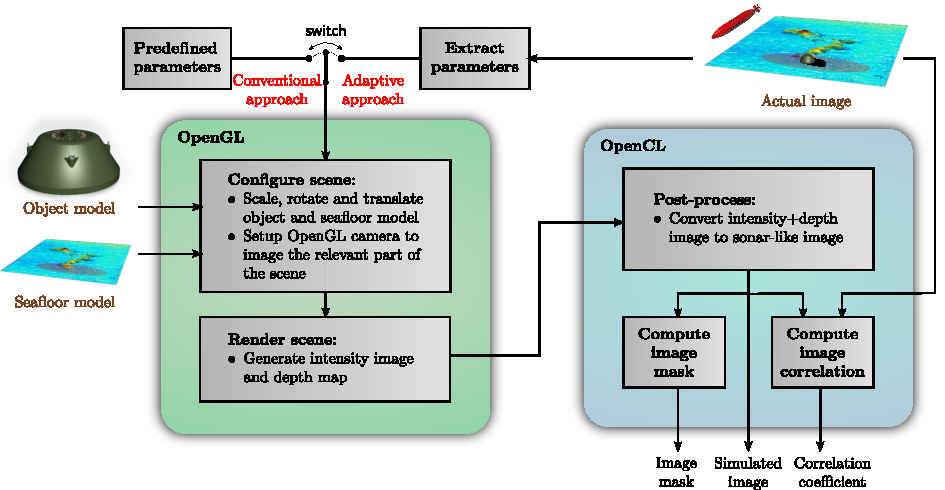
\includegraphics[width=1.25\linewidth]{gfx/simulator.pdf}}%
\else
\ifOverLeaf%
  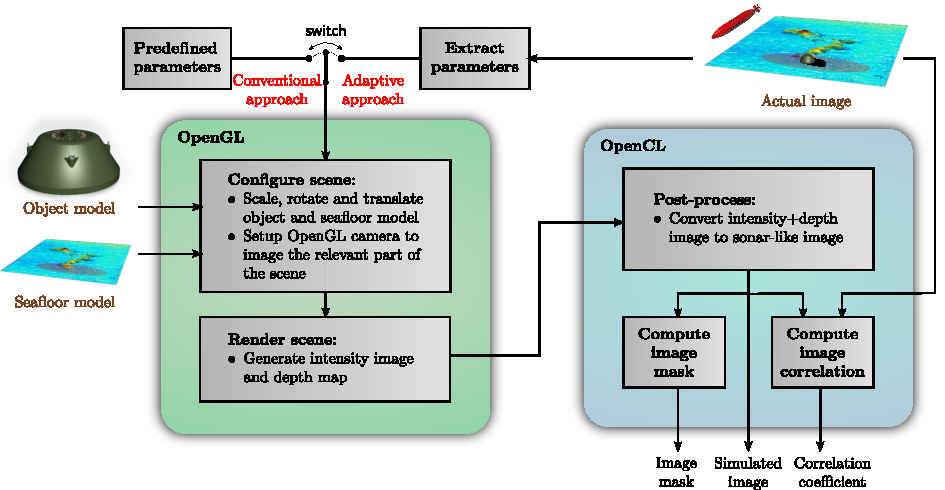
\includegraphics[width=\linewidth]{gfx/simulator.pdf}%
\else
  \includegraphics[drawing,width=\linewidth]{gfx/simulator.svg}%
\fi\fi
\caption{\emph{Simulator concept}: Given as input 3D models of the object and seafloor with some parameters for these, the simulator produces an image template, mask and a correlation coefficient. The \emph{conventional} (static) approach picks parameters from a predefined set, whereas the \emph{adaptive} approach estimates them from the sonar image. The implementation resides entirely on the GPU, with OpenGL performing scene rendering and OpenCL general-purpose post-processing. Compared to a CPU, the GPU's superior processing speed allows a much wider range of object parameters to be searched for an optimal template, yielding better results in less time.}\label{IV_buildup}%
\end{figure*}

\ifPhdDoc
\newcommand\checkicon{\includegraphics[height=2ex]{gfx/icon_check.pdf}}
\newcommand\crossicon{\includegraphics[height=2ex]{gfx/icon_cross.pdf}}
\else
\newcommand\checkicon{\includegraphics[height=2ex]{gfx/icon_check.svg}}
\newcommand\crossicon{\includegraphics[height=2ex]{gfx/icon_cross.svg}}
\fi
% \newcommand\figstep[2]{\raisebox{.5pt}{\textcircled{\raisebox{-.9pt}{\textbf{#1}}}}\mbox{}\hfill\parbox[t]{.97\linewidth}{#2}}
\ifPhdDoc
\begin{figure*}[tbp]\centering%
%    \begin{narrow}{-.125\linewidth}{-.125\linewidth}
   \captionsetup{width=1.3\linewidth,font=scriptsize}
   \makebox[\linewidth][c]{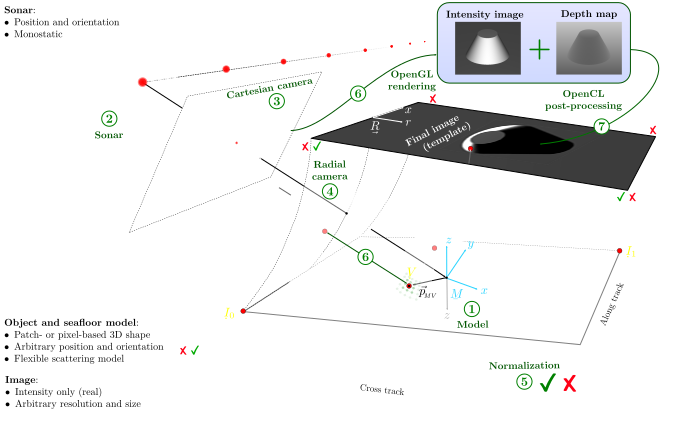
\includegraphics[width=1.3\linewidth]{gfx/scene_coordinate_system_radial.pdf}}%
   \renewcommand\emph[1]{\mdseries{#1}}
   
\else
\begin{figure*}[t]\centering%
   \ifOverLeaf%
      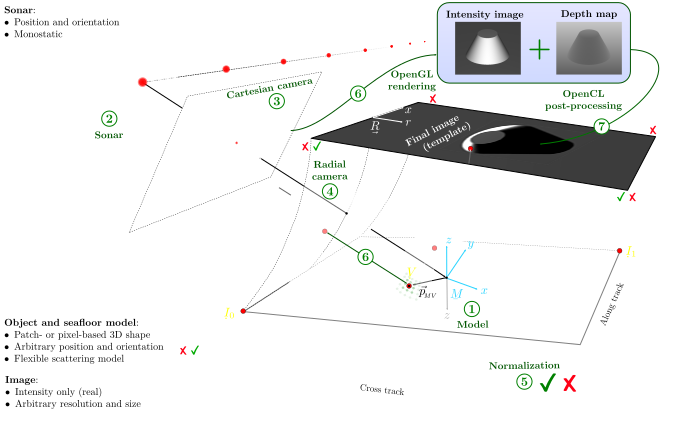
\includegraphics[width=\linewidth]{gfx/scene_coordinate_system_radial.pdf}%
   \else
      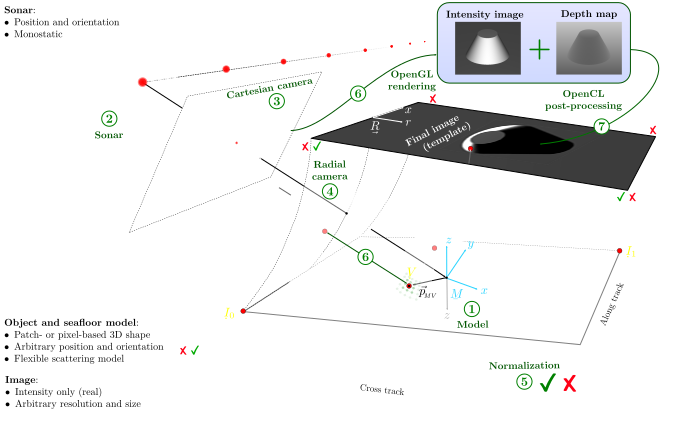
\includegraphics[width=\linewidth]{gfx/scene_coordinate_system_radial.svg}%
   \fi
\fi
\ifPhdDoc
\FloatBarrier
\fi

\caption[caption]{\emph{Virtual scene geometry and processing steps.} As marked with encircled numbers in the figure, seven steps are needed to obtain the sonar template:\\[.5\baselineskip]
%
\figstep{1}{\emph{Model displacement.} When 3D models of the seafloor and object are loaded into OpenGL, each has its own reference frame $\protect\ubar{M}$. The region we seek to image has a position and orientation $\ubar{I}$. We apply the displacement (translation and rotation) $\ubar{M} \to \ubar{I}$ with a \emph{model matrix} $\mat{T}_\textit{\tiny\!IM}$.
}\\[.5\baselineskip]
%
\figstep{2}{\emph{Sonar translation.} The sonar local body has the reference frame $\ubar{S}$. We set its orientation equal to that of the image, $\uvec{S}=\uvec{I}$, and apply the remaining translation of $\udot{I} \to \udot{S}$ with a \emph{sonar matrix} $\mat{T}_\textit{\tiny\!SI}$.
}\\[.5\baselineskip]
%
\figstep{3}{\emph{Cartesian camera rotation.} To see the world as the sonar does, we position the OpenGL camera at the origin of the sonar frame, $\udot{C}=\udot{S}$, lock its horizontal axis to that of the sonar, $\hat{x}_C=\hat{x}_S$, and direct it at the origin of the image frame, $\hat{z}_C\parallel\vec{p}_{SI}$. Since the position is correct after step 2, we apply the remaining rotation $\uvec{S} \to \uvec{C}$ with a \emph{Cartesian camera matrix} $\mat{T}_\textit{\tiny\!CS}$.
}\\[.5\baselineskip]
%
\figstep{4}{\emph{"Range" camera coordinate conversion.} The $\hat{x}_C$ and $\hat{y}_C$ axes span an orthogonal viewing plane onto which the scene's points can be projected. However, to simplify the boundary specification of range and elevation in the next step, we convert the coordinate representation from Cartesian to "ranged" (cylindrical) with a non-linear function T$_{RC}\colon (\hat{x}_C,\hat{y}_C,\hat{z}_C) \to (\hat{x}_R,\hat{\phi}_R,\hat{r}_R)$ subject to $\hat{x}_R=\hat{x}_C$.
}\\[.5\baselineskip]
%
\figstep{5}{\emph{Normalization of coordinates}. OpenGL only renders coordinates in the range $[-1,1]$. We map valid range for along-track, range and elevation (the volume marked by \checkicon{}\!s inside and \crossicon{}s outside) into this normalized range with a \emph{normalization matrix} $\mat{T}_\textit{\tiny\!NR}$.
}\\[.5\baselineskip]
%
\figstep{6}{\emph{OpenGL rendering.} When OpenGL renders the scene, it uses a \emph{vertex shader} to apply our transformation matrices to every vertex and a \emph{fragment shader} to compute the intensity values for each point in the image. OpenGL computes the range from each image pixel to its corresponding model facet: this is called a \emph{depth map}.
}\\[.5\baselineskip]
%
\figstep{7}{\emph{OpenCL post-processing.} Finally, the sonar-like image is formed---for some unique azimuth coordinate---by accumulating all intensity values that share the same range. This is our template. %  along with the depth information is finally combined to form a sonar like image. This is our template.
}%
% }
}\label{IV_simulator_coordinate_system}
\ifPhdDoc
% \end{narrow}
\fi
%
\end{figure*}

% \IEEEPARstart{W}{hen} 
% Autonomous underwater vehicles (AUVs). When an AUV with a sonar imaging system encounter an interesting object, it would be very beneficial if adapted its behavior to examine the object further. This is challenging as it would need to learn in what ways the interesting objects differ from the background, i.e. it relies on previous knowledge. It would also need to process this information is near real-time to act in an efficient manner.

% - Adapt simulation to its behaviour, see if they still match.

\IEEEPARstart{A}{utonomous} underwater vehicles (AUVs) are vital in the exploration of underwater frontiers. When equipped with a modern synthetic aperture sonar (SAS), they map seafloors, survey underwater biology, help localize wrecks, inspect oil pipes, fields and electricity lines, or help remove mines, biohazard waste or plastic. However, they struggle to deal with unforeseen events, such as poor imaging conditions, blocked paths, corrupted data or rare objects. One reason is their lack of a reliable and adaptive system for automatic target recognition (ATR).

%However, Such independent systems have much to gain from being able to adapt to the scenario at hand. For instance, with a well designed automatic target recognition (ATR) system on board they can adapt their mission plan to collect more information on particularly interesting objects, or fine-tune the sonar and navigation system to create better images.
 
% Automatic target recognition (ATR) is an important component in autonomous underwater vehicles (AUVs), as it allows the vehicle to adapt its mission plan to e.g. revisit detected objects for closer examination. One way to classify these objects is by using template matching. The principle involved  is to isolate an image segment containing the object of interest, compare it with a set of template images of the relevant object classes, and assign it to the class of the template with the the best fit.

A conventional ATR system isolates an object of interest, extracts its key features, and uses these to estimate the object's class. The challenge is to find features that are unique and intrinsic, such as type, shape and size, independent of extrinsic ones such as alignment, burial depth, degeneration level or view angle. Such features are rare in SAS, despite its best-in-class resolution and dynamic range, due to image ambiguities from acoustical distortions such as layover, multiple scattering, diffraction, dispersion and penetration.


Template matching offers an alternative to feature extraction: to compare the object with image templates of relevant classes and orientations, and assign the object to the class that fits best. The problem is finding a set of templates that properly represent the objects. Too many templates are needed to densely sample each degree of freedom. Therefore, practical implementations resort to a few sparsely sampled features, ultimately yielding inaccurate results~\cite{Midelfart2010}.


Adaptive template matching is a hybrid solution: to extract the most reliable statistics from the image, such as shadow and highlight characteristics, then use these to limit the template solution space~\cite{Midelfart2010}. This enables a fine-grained search through more features, at a reduced computational load and improved accuracy. However, we can remove a template library completely by simulating templates on-the-fly.

%, to adapt to much broader scenarios.


% estimates some To overcome the limitation on In previous work we propose to adaptive  implement adaptive template matching using partial feature extraction. 
%We implement a hybrid solution by selecting a template based on object and seafloor parameters estimated from the SAS image~\cite{Midelfart2010}.
%
%We address the efficiency and problems of conventional template matching with \emph{adaptive template matching}---selecting a template based on object and seafloor parameters estimated from the SAS image~\cite{Midelfart2010};\todo{   **template selection based on object and seafloor parameters from SAS image***       Takes up a bit too much space, considering it won't be described in great detail} and
%\emph{real-time template simulation}---creating a template tailored to the estimated parameters, to improve its accuracy and avoid the need of a precomputed template library. 

%
%\todo{However, only a few simulators for high frequency, side-looking sonar imagery have been published. ***}
A few simulators for high frequency, side-looking sonar imagery have been published, e.g.~\cite{Bell1997,Sammelm2003}. We seek a fast simulator for creating simple templates, but most implementations prioritize accurate acoustic modeling at the expense of execution speed. One exception is the SIGMAS+ simulator~\cite{Coiras2009a, Coiras2009b}, which is accelerated by the parallel computing power of graphics processing units (GPUs). Aligning with our goals, it assumes Lambertian scattering and creates the sonar image from a 3D model with multiple renderings by the OpenGL computer graphics library. However, it includes stochastic effects such as ambient noise, which we deem irrelevant for templates, and its OpenGL-centric nature makes it suboptimal as an adaptive template matcher.

%while we consider templates deterministic. Neither is

%is intended for computer graphics; a side-effect of OpenGL due to the limitations of OpenGL, which is intended for computer graphics.

%It also relies on multiple  rendering passes to create the sonar image\\

% Since OpenGL is primarily intended for computer graphics, This is a drawback of OpenGL, which leaves a lot to be desired in terms of flexibility and extensibility---OpenGL is not a general-purpose programming tool.\todo{Trim, too verbose}

% - lack of flexibility
% - lack of extensibility

% - 
% This enables fast and flexible general-purpose computing on the GPU.
% This allows tailoring the sonar image with greater flexibility and allows tighter integration with the classifier.\todo{Too vague} 
% on a new full geometrical implementation of the simulator.

Our simulator was designed from the ground up to be part of a GPU-accelerated adaptive template matcher. It uses both OpenGL and the general-purpose programming framework OpenCL; two libraries that can inter-operate on the GPU. We describe it using a new notation system for homogeneous coordinates that allows complicated geometries to be expressed in a rigorous, unified and simple way. Its function is verified using data from Jesus Bay, Norway, recorded by the HISAS1030 100\,kHz SAS  mounted on a HUGIN AUV from Kongsberg Maritime.



\section{Methods}\label{IV_methods}


%
\ifPhdDoc
\begin{table*}[t]\centering
\newlength\numhspace\setlength\numhspace{-0.4em}
\newlength\labelvspace\setlength\labelvspace{-20pt}
\else
\begin{table*}[thbp]\centering
\newlength\numhspace\setlength\numhspace{-0.9em}
\newlength\labelvspace\setlength\labelvspace{-12pt}
\fi
%
{
\newcommand\shiftup[1]{\raisebox{-.75\normalbaselineskip}{#1}}
\newcommand\shiftdown[1]{\smash{\raisebox{.75\normalbaselineskip}{#1}}}
\newcolumntype{L}{>{\collectcell\shiftdown}l<{\endcollectcell}}
\newcolumntype{C}{>{\collectcell\shiftdown}c<{\endcollectcell}}
\newcolumntype{O}{>{\collectcell\shiftdown\hspace*{-1.75\tabcolsep}}l<{\endcollectcell}}
\newcolumntype{Q}{>{\collectcell\shiftdown\hspace*{-1.75\tabcolsep}}c<{\endcollectcell}}
\newcolumntype{P}[1]{>{\collectcell\shiftdown}p{#1}<{\endcollectcell}}
\providecommand\t*{}\renewcommand*\t[1]{{\tikzmark{#1}{$\ubar{#1}$}}}
%	\hline\hspace*{-1.75\tabcolsep}
%\newcolumntype{L}[1]{>{\raggedright\let\newline\\\arraybackslash\hspace{0pt}}m{#1}}
%\newcolumntype{C}[1]{>{\centering\let\newline\\\arraybackslash\hspace{0pt}}m{#1}}
%\newcolumntype{R}[1]{>{\raggedleft\let\newline\\\arraybackslash\hspace{0pt}}m{#1}}
%%
\def\arraystretch{1.5}
% \setlength{\belowrulesep}{0pt}
%\setlength{\extrarowheight}{0.5ex}
\newcommand\pt[1]{\parbox[c]{1.5em}{text}}
%\cellcolor[gray]{.9}
\newcommand\mc[3]{\multicolumn{#1}{#2}{#3}}
\providecommand*\T{}\renewcommand*\T[1]{\parbox[l]{2em}{$\vec{T}_{#1}$}}
%\providecommand*\Tr{}\renewcommand*\Tr[1]{\parbox[l]{3em}{$\dvec{T}_{#1}($}\parbox[l]{3em}{#2}\parbox[l]{3em}{#3}\parbox[l]{0.75em}{#4})}
\providecommand*\Tr{}\renewcommand*\Tr[1]{$\dvec{T}_{#1}$}
\providecommand*\inn{}\renewcommand*\inn[1]{}%\in\mathrm{#1}(3)}
\providecommand*\TT{}\renewcommand*\TT[1]{\parbox[l]{2em}{T$_{#1}$}}
\providecommand*\p{}\renewcommand*\p[2]{\parbox[l]{2em}{$\dvec{p}_{#1}^{#2}$}}
\providecommand*\SIM{}\renewcommand*\SIM{$\mathrm{Sim}(3)$}
\providecommand*\SE{}\renewcommand*\SE{$\mathrm{SE}(3)$}
\providecommand*\Emph{}\renewcommand*\Emph[1]{\shiftup{\emph{#1}}}
\newcommand{\REmph}[1]{\tikz[remember picture,baseline=(#1.base)]\node[transform canvas={yshift=.75\normalbaselineskip},align=center,rotate=30,inner sep=0pt](#1){#1};}
%\newcommand{\trot}[1]{\tikz[remember picture,baseline=(#1.base)]\node[shape=rectangle,inner sep=0pt](#1){#1};}
%\newcommand{\tikzmark}[2]{\tikz[remember picture,baseline=(#1.base)]\node[shape=rectangle,inner sep=0pt](#1){#1};}
% \node(ACe)[below = 2\baselineskip of CC, anchor=center]%
%    {\footnotesize\textrm{Change of vector}};
%\setlength{\tabcolsep}{1.5em} @{\extracolsep{0em}}
\newcommand\mcc[3]{\mc{#1}{#2}{\shiftup{#3}}}
%\providecommand*\REmph{}\renewcommand*\REmph[1]{{A}}%\raisebox{-1.5ex}{\rotatebox{25}{\emph{#1}}}}}
\newcommand\addtimes{\hspace*{1.92\tabcolsep}\makebox[0pt]{,}\hspace*{-1.92\tabcolsep}}
\newcommand\addtimess{\hspace*{\tabcolsep}\makebox[0pt]{$\times$}\hspace*{\tabcolsep}}
\newcommand\addin{\hspace*{\tabcolsep}\makebox[0pt]{$\in$}}
\newcommand\const[1]{%\cellcolor{black!64}
#1}
%
\ifPhdDoc
\makebox[\linewidth][c]{\resizebox{1.25\linewidth}{!}{
\fi
%(\cdot)\\[-.75\normalbaselineskip]\cmidrule(lr){3-20}\\[-0.75\normalbaselineskip]\rowcolor{tabBlue}-1.15em}
\begin{tabular}{r c >{\hspace*{\numhspace}} C >{\hspace*{0.5em}} O Q >{\hspace*{-.5em}} Q Q Q C O C C C L >{\hspace*{-2\tabcolsep}}L O O O >{\hspace*{\tabcolsep}} O O O >{\hspace*{\tabcolsep}}  O O @{\hspace*{\tabcolsep}\shiftdown{$\in$}\hspace*{\tabcolsep}} L}
	\topline\rowcolor{cBase}
   \mc{2}{c}{\bf Frame} & & \mc{5}{c}{\bf Transformation} & \mc{5}{c}{\bf Configuration space} & \mc{11}{c}{\bf Representation} \\
   \cmidwrap{\cmidrule(lr){1-2}\cmidrule(lr){3-8}\cmidrule(lr){9-13}\cmidrule(lr){14-24}}\rowcolor{cBase} 
	\emph{Description} & \emph{Symbol} & \Emph{} & \Emph{$\vec{T}$} & \mc{4}{O}{\Emph{$\colon$ Mapping}} & \Emph{$\mathcal{C}($} & \Emph{$\vec{p}$\addtimes} & \Emph{$\vec{R}$\addtimes} & \Emph{$s)$} &  \Emph{DoF$^{(1)}$} &  \mc{1}{l}{\emph{$\mat{T}$}} & \Emph{$($} & & \Emph{$\dvec{p}$} & \Emph{$\phantom{z},$}  & & \Emph{$\dvec{R}$} & \Emph{$\phantom{\phi},$} &  \Emph{$s$} & \mc{1}{>{\hspace{-1.75\tabcolsep}}l}{$)$} & \Emph{Group} \\%\Emph{Sum} \\
	\midline
	                                         Model & \t{M}             &&                                             &          &            &       &                           &  &                &           &                &   & \mcc{1}{L}{}      &                                                                      &      &      &      &         &           &         &     & \mcc{1}{C}{} &      \\
	                                         Image & \t{I}             &\figstep{1}{}& \T{IM}                                      & $\colon$ & $\ubar{M}$ & $\to$ & $\ubar{I}$                &  & $\mathbb{R}^3$ & $S^2 S$ & $\mathbb{R}^+$ & 7 & \Tr{IM}           & $($                                                                  & $x,$ & $y,$ & $z,$ & $\psi,$ & $\theta,$ & $\phi,$ & $s$ & $)$          & \SIM \\
	                                         Sonar & \t{S}             &\figstep{2}{}& \T{SI}                                      & $\colon$ & $\udot{I}$ & $\to$ & $\udot{S}$                &  & $\mathbb{R}^3$ &         &                & 3 & \Tr{SI}           & $($                                                                  & $x,$ & $y,$ & $z$ &  &  & &     & $)$          & \SE  \\
	                                         Cartesian camera & \t{C}             &\figstep{3}{}& \T{CS}                                      & $\colon$ & $\uvec{S}$ & $\overset{(2)}{\to}$ & $\uvec{C}$ &  &                & \phantom{$S$}     &                & 0 & \Tr{CS}           & $($                                                                  &      &      &      & $\psi$\makebox[0pt][l]{$^{(2)}$}  &           &         &     & $)$          & \SE  \\
                              
\cmidrule{14-24}\rowcolor{cBase}
   \mc{13}{L}{\cellcolor{white}\hspace{16.7em}\raisebox{\labelvspace}{\color{cBaseMark}\begin{tabular}{l l}\rowcolor{white}
   $\Uparrow$ & \emph{Affine manipulations} \\$\Downarrow$ & \emph{Coordinate manipulations}
   \end{tabular}}} & \mc{1}{l}{\emph{$\mat{T}$}}                 & \mc{9}{O}{\hspace*{0\tabcolsep}\Emph{$\colon$ Mapping}} &  \\\arrayrulecolor{cBaseMark}\hline\arrayrulecolor{black}%cline{10-20}
	                                               &                    \\[0\baselineskip]
	                                Radial camera & \t{R}             &\figstep{4}{}&                                             &                             & & &                 &  &                &           &                &   & \mc{11}{L}{\hspace*{-\tabcolsep}\begin{tabular}[c]{p{2.2em} @{ $\colon$} p{7em} @{ $\to$ } p{3.45em} @{ $\in$ } l} $T_{RC}$ & $(x,y,z)   \in\mathbb{R}^3$          & $(x,\varphi,r)$ &  $\mathbb{R}S\mathbb{R}$ \end{tabular}} \\
	                                      Normalized coordinates & \t{N}             &\figstep{5}{}&                                             &                             & & &                 &  &                &           &                &   & \mc{11}{L}{\hspace*{-\tabcolsep}\begin{tabular}[c]{p{2.2em} @{ $\colon$} p{7em} @{ $\to$ } p{3.45em} @{ $\in$ } l} \Tr{NR}           & $(x,\phi,r)\in\mathbb{R}S\mathbb{R}$ & NDC$^{(3)}$  &  $[0,1]^3$ \end{tabular}} \\ \bottomrule
                                         %\end{tabular}\parbox[L]{8em}{} $\to$ \parbox[L]{3.8em}{NDC$^{(3)}$} \parbox[L]{1em}{$\in$} $[0,1]^3$}   \\ \bottomrule
\mc{10}{l}{$^{(1)}$Degrees of Freedom} \\
\mc{10}{l}{$^{(2)}$Subject to $\hat{x}_C = \hat{x}_S$ and $\hat{z}_C \parallel \vec{p}_{SI}$} \\
\mc{10}{l}{$^{(3)}$Normalized Device Coordinates}
%\mc{10}{l}{$^{(4)}$Subject to $\hat{x}_O = \hat{x}_S$ and $\hat{z}_O \parallel \vec{p}_{SI}$}
\end{tabular}
%	                                Cylindric view & \t{C}             &                                             &                                               &  &                &           &                &   & $\mathrm{T}_{RC}$ & \mc{8}{O}{\hspace*{0\tabcolsep}$\colon (x,y,z)\in\mathbb{R}^3$}&\mc{1}{O}{$\to (x,\phi,r)\in$}&$\mathbb{R}S\mathbb{R}$   \\
%	                                      Clipping & \t{X}             &                                             &                                               &  &                &           &                &   & \Tr{NR}           & \mc{8}{O}{\hspace*{0\tabcolsep}$\colon (x,\phi,r)\in\mathbb{R}S\mathbb{R}$}&\mc{2}{O}{\hspace*{-\tabcolsep}$\to [0,1]^3$}   \\ \bottomrule
%	                 \mc{10}{l}{$^{(1)}$Degrees of freedom} &  \\
%
%cartesian $\rightarrow$ cylindric
%orthographic projection
%\p{MV}{M}
%\p{IV}{I}
%\p{SV}{S}
%& \p{OV}{O}
%\p{CV}{C}
%\p{XV}{X}
\begin{tikzpicture}[overlay,color=cBaseMark,remember picture, shorten >=-3pt]
%
\tikzset{
  c/.style={
    anchor=south west,
    node font=\itshape,
%    draw,
    align=center,
    rotate=30,
    yshift=-.2ex,
    xshift=-0.5em,
    align=left
  }
}
%\node[c] at (Rot){\rotatebox{0}{Rotation}};
%\node[c] at (Tra){\rotatebox{0}{Translation}};
%\node[c] at (Sca){\rotatebox{0}{Scale}};
%\node[c] at (Sum){\rotatebox{0}{DoF}};
%\node[anchor=base,transform canvas={yshift=.75\normalbaselineskip},align=left,rotate=30,inner sep=0pt](Rot){Rotation};
%\draw[->] ($(M.center) - (1.3em,0ex)$) to[out=-90, in=90] ($(O.center) - (1.3em,-.7ex)$);
\coordinate(IM) at ($(I)!0.5!(M)$);
\coordinate(SI) at ($(S)!0.5!(I)$);
\coordinate(CS) at ($(C)!0.5!(S)$);
\coordinate(RC) at ($(R)!0.5!(C)$);
\coordinate(NR) at ($(N)!0.5!(R)$);
\coordinate(offset) at (0.5em,0ex); %5.3em
%\path let \p1 = (TL.west), \p2 = (RC) in coordinate (SW) at (\x1,\y2);
%\path let \p1 = (TL.east), \p2 = (RC) in coordinate (SE) at (\x1,\y2);
%\node[anchor=base,text width=\minWidth,align=\alignment,inner sep=0pt,inner xsep=\tabcolsep,outer sep=0pt] (n) {\strut$#1$}
%\node(affine)[left = 5.6em of IM, anchor=center]{\footnotesize\textrm{Affine}};
%\node(affine)[left = 5.6em of SI, anchor=center]{\footnotesize\textrm{Affine}};
%\node(affine)[left = 5.6em of CS, anchor=center]{\footnotesize\textrm{Affine}};
%\node(nonlin)[left = 5.6em of RC, anchor=center]{\footnotesize\textrm{Non-linear}};
%\node(project)[left = 5.6em of NR, anchor=center]{\footnotesize\textrm{Projective}};
% \node(step1)[anchor=center] at ($(X)+(2.8em,-0.2em)$){\figstep{1}{}};
%\draw[-]
%                        (FrameL.south) to[out=0, in=180] (FrameR.south);
\draw[-{Latex[length=.5em,width=.5em]}]
                        ($(R.center) + (offset) + (1.3em,-0.4ex)$) to[out=-30, in=90] ($(NR) + (offset) + (1.6em,0ex)$)
      to[out=-90, in=0] ($(N.center) + (offset) + (0.8em,0ex)$);
\draw[-{Latex[length=.5em,width=.5em]},draw,densely dotted]                
                        ($(C.center) + (offset) + (1.1em,-0.4ex)$) to[out=-45, in=90] ($(RC) + (offset) + (1.6em,0ex)$)
      to[out=-90, in=0] ($(R.center) + (offset) + (0.8em,0ex)$);
\draw[-{Latex[length=.5em,width=.5em]}]
                        ($(S.center) + (offset) + (1.3em,-0.4ex)$) to[out=-30, in=90] ($(CS) + (offset) + (1.6em,0ex)$)
      to[out=-90, in=0] ($(C.center) + (offset) + (0.8em,0ex)$);
\draw[-{Latex[length=.5em,width=.5em]}]
                        ($(I.center) + (offset) + (1.3em,-0.4ex)$) to[out=-30, in=90] ($(SI) + (offset) + (1.6em,0ex)$)
      to[out=-90, in=0] ($(S.center) + (offset) + (0.8em,0ex)$);
\draw[-{Latex[length=.5em,width=.5em]}]
                        ($(M.center) + (offset) + (0.44em,0ex)$) to[out=0, in=90] ($(IM) + (offset) + (1.6em,0ex)$)
      to[out=-90, in=0] ($(I.center) + (offset) + (0.8em,0ex)$);
%\draw[-{Latex[length=.5em,width=.5em]}]
%                        ($(M.center) + (offset) + (0.44em,0ex)$) to[out=0, in=90] ($(IM) + (offset) + (1.6em,0ex)$)
%      to[out=-90, in=0] ($(I.center) + (offset) + (0.44em,0ex)$) to[out=0, in=90] ($(SI) + (offset) + (1.6em,0ex)$);
%      to[out=-90, in=0] ($(S.center) + (offset) + (0.44em,0ex)$) to[out=0, in=90] ($(CS) + (offset) + (1.6em,0ex)$)
%      to[out=-90, in=0] ($(C.center) + (offset) + (0.8em,0ex)$);
%%\path[fill=gray,opacity=0.2](TL.north east)--(TL.north east)--(SE)--cycle;
%%%%\draw[->] ($(I.east) - (.7em,0ex)$) to[out=-180, in=180] ($(S.east) - (.7em,0ex)$);
%%%%\draw[->] ($(S.east) - (.7em,0ex)$) to[out=-180, in=180] ($(C.east) - (.7em,0ex)$);
%%%%\draw[->] ($(C.east) - (.7em,0ex)$) to[out=-180, in=180] ($(R.east) - (.7em,0ex)$);
%%%%\draw[->] ($(R.east) - (.7em,0ex)$) to[out=-180, in=180] ($(X.east) - (.7em,0ex)$);
%%%%\draw[->,yshift=2ex] (pic cs:M) -- (pic cs:I) ;
\end{tikzpicture}
\ifPhdDoc
}}
\fi
}
\caption{Reference frames and their transformations. The upper half is an affine domain where any pair of frames are related by a displacement with a specific configuration and a chosen coordinate representation. The lower half is a domain where frames represent intermediary states between coordinate manipulations. All set-multiplications are cartesian.}\label{IV_tab_frames_transitions}
\end{table*}

\Fig{IV_buildup} illustrates the basic idea behind the simulator: to use OpenGL to render an intensity and depth image of an object and seafloor model, and OpenCL to convert these into an image template. We call the method conventional when its input parameters are predefined, and adaptive when they are estimated from the SAS image.


% Depending on whether the input parameters are predefined or estimated from the SAS image, the use the label conventional or adaptive approach, respectively.

\Fig{IV_simulator_coordinate_system} and \Tab{IV_tab_frames_transitions} detail the geometry and processing steps that underpin most of the upcoming implementation details. The steps first detail the transformations a vertex $\udot{V}$ undergoes---from being represented in the reference frame of a model, $\ubar{M}$, to that of an OpenGL camera, $\ubar{C}$---then discuss rendering and post-processing details. The mathematical syntax comes from a rigorous navigational notation system and rule set developed by K.~Gade~\cite{Gade2018}, which has a free and decomposed form.
%be rthat of the image region  $\ubar{I}$ , a sonar $\ubar{S}$, an orthogonal and cylindric viewing plane, $\ubar{O}$ and $\ubar{C}$ respectively, and a clipping space $\ubar{N}$ (not shown in \Fig{IV_simulator_coordinate_system}).\todo{Not sure if about this sentence.}


The free form emphasizes geometrical reasoning, conceptual clarity and physical understanding, while the decomposed form ensures geometrical validity and clarity when constructing, manipulating and interpreting coordinates. Together they help the designer focus on higher level concepts rather than getting lost in implementation details, such as mixing coordinates from different frames.%, such as ensuring that a vectors rather than ensuring that the points are decomposed in the same frame).
%
% and ing,  coordinates; manipulating them can be tricky and tedious, their interpretation ambiguous, and their construction error prone. Strict discipline is needed to avoid constructing invalid geometrical operations, such as mixing coordinates from two different frames. The notation aids system unambiguously expresses geometrical meaning and validity, thus allowing the designer to focus on higher level concepts rather than getting lost in implementation details. 

We adhere to Gade's notation for affine geometry, extend it to handle homogeneous coordinates and projective geometry, and suggest a slight tweak for arbitrary functions. This facilitates transitioning between frames in a unified and geometrically valid way. Inspired by modern robotics, we also discuss the topology and Lie group theory of rigid objects~\cite{Lynch2017}. 




\subsection{Free notation}\label{IV_sec:general_notation}


Suppose a stationary $N$-dimensional rigid model has a reference frame $\ubar{M} \triangleq (\udot{M},\uvec{M})$ attached to it, where $\udot{M}\in\mathbb{A}$ is its absolute position and $\uvec{M}\triangleq\big(\hat{x}_{M},\hat{y}_{M},\dots\big)\in\mathbb{V}^N$ its absolute orientation (where $\hat{\cdot}$ denotes unit length).
%
%
%
%The set of all possible configurations for the model is called its C-space, its dimension matching the number of degrees of freedom and its shape matching the topology. Rigid bodies have $N(N+1)/2$ degrees of freedom, $N$ Euclidean ones for position (topology $\mathbb{E}^N$), and $N(N-1)/2$ angular ones for orientation (topology $S^2S^1$ or $S^1$ for $N=\{3,2\}$, respectively).
%
%
A vertex $\udot{V}$ in the model can be related to the frame by a position vector $\vec{p}_{\td{M}\td{V}}\in\mathbb{V}$ going from $\udot{M}$ to $\udot{V}$,
%
\begin{align}\label{eq_p_MV_free}
\vec{p}_{\d{M}\d{V}} &\triangleq \udot{V} - \udot{M},
\end{align}
%
where $\vec{p}_{\udot{M}{V}} = -\vec{p}_{\udot{V}\udot{M}}$. 

An image frame $\ubar{I}$ specifies the location and orientation of the seafloor area where we want to place the model. We express the \emph{displacement} $\vec{T}_{\ubar{I}\ubar{M}}$ of {\color{cFrame}frame} $\ubar{M}$ relative to $\ubar{I}$,
%
\begin{align}
\vec{T}_{\bb{I}{M}} \colon \ubar{M} &\to \ubar{I},\label{eq_T_IM_free}
\intertext{in terms of a \emph{translation} $\vec{p}_{\udot{I}\udot{M}}$ that relates their {\color{cPoint}positions},}
\vec{p}_{\dd{I}{M}} \triangleq \udot{M} &- \udot{I},\label{eq_p_IM_free}
\intertext{and a \emph{rotation} $\vec{R}_{\uvec{I}\uvec{M}}$ that relates their {\color{cBasis}orientations},}
\vec{R}_{\vv{I}{M}} \colon \uvec{M} &\to \uvec{I}\label{eq_R_IM_free}\\\nonumber
\vec{m} &\mapsto \vec{i}.
\end{align}
%
% Vector subscripts define {\color{cPoint}direction} and {\color{cPoint}magnitude} in terms of two points, and superscripts define {\color{cBasis}representation} in terms of a 
% 
We can write the configuration of $\vec{T}_{\tb{I}\tb{M}}$ as $\mathcal{C}_{\tb{I}\tb{M}}=(\vec{p}_{\td{I}\td{M}},\vec{R}_{\ta{I}\ta{M}})$.
%
%%$\vec{p}_{IM}$ has $N$ degrees of freedom and Euclidean topology $\mathbb{R}^N$. $\vec{R}_{IM}$
%
%%It has $N(N+1)/2$ degrees of freedom: $N$ for the translation, and the rest for orientation. 
%The translation has $N$ degrees of freedom and topology $\mathbb{R}^N$. The rotation has $N(N-1)/2$ degrees of freedom with topology $\{S^2\times{}S^1, S^1\}$ for $N=\{3,2\}$.
%
It has $N(N+1)/2$ degrees of freedom: $N$ for the translation, with Euclidean topology $\mathbb{R}^N$; and $N(N-1)/2$ for rotation, with angular topology $\{S^2\times{}S^1, S^1\}$ for $N=\{3,2\}$. The symbol $\times$, which denotes the cartesian product of sets, will be dropped and assumed implicit in upcoming set-multiplications. We also drop the sub- and superscript accents and colors from symbols in the text, but keep it for comparison in the standalone equations. All frames and their configurations are listed in \Tab{IV_tab_frames_transitions}, along with an associated numeric representation. We describe this next.

% \dvec{p} vector subscripts define {\color{cPoint}direction} and {\color{cPoint}magnitude} in terms of two points, and superscripts define {\color{cBasis}representation} in terms of a . Stated differently, subscripts define geometric features while superscripts define numerical features.


\subsection{Decomposed notation}\label{IV_decomposed_notation}

Suppose we reference the model's vertices from the image frame $\ubar{I}$ using the head-to-tail vector rule,
%
\begin{align}\label{IV_eq_free_vector_addition}
\m{CL}
\vec{p}_{\dd[IV]{I}{V}}
= \vec{p}_{\d[I]{I}\cd[M1]{M}}
+ \vec{p}_{\cd[M2]{M}\d[V]{V}},
\m{CR}
\\\nonumber
\tikz[overlay,remember picture]{
  % Set up some general bounding box markers
%  \coordinate(IV)  at ($ .5*(I1.south) + .5*(V1.south)  $);
  \coordinate(_MV) at ($    (V.south)  + (-1.0\baselineskip,-1.0\baselineskip) $);
  \coordinate(_IV) at ($    (IV.south) + ( 1.0\baselineskip,-1.0\baselineskip) $);
  \coordinate(_IM) at ($    (I.south)  + (-1.0\baselineskip,-1.0\baselineskip) $);
  \coordinate(_IV_IM) at ($ .5*(_IV) + .5*(_IM) $);
  % Draw arrows and text
    \draw[color=cBrightArrow]  ($ (V.south)  - (0em,\tpad) $)
            to[out=-90, in=0]     (_MV)
            to[out=180, in=0]     (_IV_IM)
            to[out=180, in=-90]($ (IV.south) - (0em,\tpad) $);
    \draw[-,color=cBrightArrow]($ (I.south)  - (0em,\tpad) $)
            to[out=-90, in=0]     (_IV_IM);
    }
\end{align}
%
where $\c[M]{M}$ denotes cancellation of the intermediate frame $\ubar{M}$ and arrows emphasize composition of the output vector.
This vector addition (and any other vector-vector operation) is numerically possible and valid if---and only if---all vectors are decomposed, or represented, in the same frame. Since position vectors have Euclidean topology, we represent $\vec{p}$ in $\ubar{I}$ with a real number for each degree of freedom, $\dvec{p}^{I}\in\mathbb{R}^N$, and unambiguously rewrite \eq{IV_eq_free_vector_addition} in decomposed form as
%
\begin{align}
\m{CL}
\dvec{p}_{\d[IV]{IV}}^{\,\v[I1]{I}} &= \dvec{p}_{\d[II1]{I}\cd[M1]{M}}^{\,\v[I2]{I}} + \dvec{p}_{\cd[M2]{M}\d[V1]{V}}^{\,\v[I3]{I}},\label{eq_head_tail_decomposed}
\m{CR}
\\\nonumber
\tikz[overlay,remember picture]{
  % Set up some general bounding box markers
  \coordinate(_MV) at ($    (V1.south)  + (-1.0\baselineskip,-1.0\baselineskip) $);
  \coordinate(_IV) at ($    (IV.south) + ( 1.0\baselineskip,-1.0\baselineskip) $);
  \coordinate(_IM) at ($    (II1.south)  + (-1.0\baselineskip,-1.0\baselineskip) $);
  \coordinate(_IV_IM) at ($ .5*(_IV) + .5*(_IM) $);
  % Draw arrows and text
    \draw[color=cBrightArrow]      ($ (V1.south)  - (0em,\tpad) $)
            to[out=-90, in=0]     (_MV)
            to[out=180, in=0]     (_IV_IM)
            to[out=180, in=-90]($ (IV.south) - (0em,\tpad) $);
    \draw[-,color=cBrightArrow]    ($ (II1.south)  - (0em,\tpad) $)
            to[out=-90, in=0]     (_IV_IM);
    }
\end{align}
%
% Inverse $\dvec{R}^{-1} = \dvec{R}^T$\\
% Closure $\dvec{R}_1\dvec{R}_2 \in\mathrm{SO(3)}$\\
% Associative but not commutative
% <<
% 
where bold symbols without accents denote decomposed elements such as vectors and matrices. 

To obtain $\dvec{p}_{MV}^I$ we must rotate $\dvec{p}_{MV}^M$ by $\vec{R}_{IM}$. Since rotations have angular topology, we represent them in a space with more dimensions than degrees of freedom, which avoids issues with rapidly changing values and singularities (e.g. Gimbal lock). A common choice is a rotation matrix $\dvec{R}\in\mathrm{SO}(N)$, i.e. a special (right handed) orthogonal $\mathbb{R}^{N\times{}N}$ matrix, with the properties $|\dvec{R}|=1$ (left-handed would be $-1$) and $\dvec{R}^T\dvec{R} = \dvec{R}\dvec{R}^T = \dvec{I}$. The latter property constrains the column vectors of $\dvec{R}$ to be independent (orthogonal) and of unit length. This leaves $\dvec{R}$ with $N(N-1)/2$ degrees of freedom, as desired. Thus, a suitable representation of $\vec{R}_{IM}$ in $\uvec{I}$ is $\dvec{R}_{IM}^I = \dvec{R}_{IM}\in \mathrm{SO}(N)$, subject to $\uvec{M} \mapsto \uvec{I}$,
%
\begin{align}\nonumber\\
\m{CL}
\dvec{p}_{\dd[MV1]{M}{V}}^{\,\v[I1]{I}}
= \mat{R}_{\v[I2]{I}\cv[M1]{M}} \; \dvec{p}_{\dd[MV2]{M}{V}}^{\c[M2]{M}}.\m{CR}
\label{eq_passive_rotation}
%
\tikz[overlay,remember picture]{
  % Set up some general bounding box markers
  \coordinate(R) at ($ .5*(CL.north)  + .5*(CR.north) + (0em,1\baselineskip) $);
  % Compute arrow via points
  \path let \p1 = ($ (I1) + (1.0\baselineskip,0em) $),  \p2 = (R) in coordinate (_I1)  at (\x1,\y2);
  \path let \p1 = ($ (I2) - (1.0\baselineskip,0em) $),  \p2 = (R) in coordinate (_I2)  at (\x1,\y2);
  \path let \p1 = ($.5*(M1) +.5*(M2)$),  \p2 = (R) in coordinate (_M)  at (\x1,\y2);
  % Draw arrows and text
%    \draw[]                  ($ (M2.north) + (0em,\tpad) $)
%           to[out= 90, in=0]    (_M)
%           to[out=180, in=90]($ (M1.north) + (0em,\tpad) $);
    \draw[color=cDarkArrow]      ($ (I2.north) + (0em,\tpad) $)
           to[out= 90, in=0]    (_I2)
           to[out=180, in=0]    (_I1)
           to[out=180, in=90]($ (I1.north) + (0em,\tpad) $);
}
\end{align}
%
When $\dvec{R}_{IM} = \bmat{\boldsymbol{\hat{x}}_M^S & \boldsymbol{\hat{y}}_M^S & \boldsymbol{\hat{z}}_M^S}$ is left-multiplied as here, we interpret it as the \emph{orientation} of $\uvec{M}$ \emph{represented} in $\uvec{I}$, and \emph{vice versa} if it is right-multiplied. Multiplication by a $\mathrm{SO}(N)$ matrix is associative, generally non-commutative and closed.  %Embee
%, and the orthogonality follows from the skew symmetry of the axis of rotation. %SO$(N)$ are also known as rigid transformations, because they preserve the distance and orientation between points~\cite{Murray1994}\footnote{Pages 26-27}\todo{Valid page specification?}.
%
We can drop the superscript, $\dvec{R}_{IM} = \dvec{R}_{IM}^I = \dvec{R}_{IM}^M$, because $\dvec{p}_{MV}^M$ is rotated around a $\mathbb{R}^{N-2}$-subspace that is fixed in both $\ubar{I}$ and $\ubar{M}$.

The rotation in \eq{eq_passive_rotation} is called passive because its geometric intent is to change the representation but leave the absolute position of the point unchanged. An active transformation, by contrast, changes the vector but not the representation. A notational remark on this can be found in Appendix \ref{IV_sec:active_passive_rotations}, but only passive transformations will be needed henceforth.


\subsection{Homogeneous transformations}

Any transformation in $\mathbb{R}^N$-space can be represented by a transformation matrix $\dvec{T} \in \mathbb{R}^{N+1,N+1}$. In the affine case, it has the form of a Special Euclidean matrix $\dvec{T}\in\mathrm{SE}(N)$,
%
\begin{align}
\dvec{T} &= 
\left[\begin{array}{c c}
 \mat{R}  & \dvec{p} \\%\hline
 \dvec{0}^T  &  1
\end{array}\right] = \mathrm{SE}(N)\label{IV_eq_T_decomposed}
\end{align}
%
where both $\mat{T}$, $\dvec{p}\in\mathbb{R}^N$ and $\mat{R}\in\mathrm{SO}(N)$ are decomposed in the same frame, and $\dvec{0}^T$ is a row zero-vector of length $N$. If the last row is altered in any way, the transform becomes real projective, $\mat{T}\in\mathbb{RP}(N)$. In any case, it shares the multiplicative properties of the rotation matrix by being associative, generally non-commutative and closed. %The regular affine version  Steps \step{1} to \step{4} 

%\eq{IV_eq_T_decomposed} contains six degrees 

As we dive into the specifics of each transformation, or step, look to \Tab{IV_tab_frames_transitions} for details on its configuration and coordinate representation, to \Fig{IV_simulator_coordinate_system} for visual aid, and to the supplementary Python script for implementation details. We use free notation in the text and decomposed notation in the standalone equations, to emphasize the merits of each. Assume the world as three dimensional and note that each step has a label in the figure, a line in the table, and a matching heading number in the upcoming text.


%  In regular world space we use the affine version in \eq{IV_eq_T_decomposed}, but the last step is performing non-linear effects \Tab{IV_tab_frames_transitions} \eq{IV_eq_T_decomposed}

%There is nothing special with this matrix, it simply combines a rotation and translation into a single operation. If the latter row 
%
%The vertex $\udot{V}$ is now referenced from $\ubar{I}$, but we prefer it referenced from the position of the sonar local body $\udot{S}$, with an orientation $\uvec{O}$ that creates a viewing plane orthogonal to $\vec{p}_{SI}$. This mimics a camera placed at the acoustic source directed at the part of the seafloor we seek to image. For this we seek the These transforms take the form of \eq{eq_homogeneous_transformation} and can be stacked together,
%%




\ifPhdDoc
\subsubsection{Model displacement}
\else
\subsubsection{Model displacement \texorpdfstring{$\vec{T}_{IM}$}{T\_IM}}
\fi

%The model is subject to no constraints 
%$\mathcal{C}_{IM} = (\vec{p}_{IM},\vec{R}_{IM},s_{IM})$, subject to no constraints, for a seven user-defined degrees of freedom.

Recall that a rigid object in three-dimensional space has six degrees of freedom: three for position and three for orientation. Consequently, for each rigid body transform, the sum of independent constraints and user-defined parameters must be six; with the exception of seven in the case of the model because we add a scaling factor $s_{IM}$ to its configuration, $\mathcal{C}_{IM} = (\vec{p}_{IM},\vec{R}_{IM},s_{IM})$. For implementation we represent $\vec{T}_{IM}\colon \ubar{M}\to\ubar{I}$ in $\ubar{I}$ by a similarity matrix,
%
%We previously found that the representation of $\mathcal{C}_{IM}$ in $\uvec{I}$ can be written $\boldsymbol{\mathcal{C}}_{IM}^I = (\dvec{p}_{IM}^I,\mat{R}_{IM})$. To allow resizing the model, we now also add a scaling factor $s_{IM}$ (see \Tab{IV_tab_frames_transitions}). 
% where Sim(3) is the set of $\mathbb{R}^{4\times4}$ similarity matrices that scales objects but otherwise preserves them (like the SE(3) group)
%
\begin{align}%\nonumber\\
\dvec{T}_{\b{I}\b{M}}^{\,\v[I1]{I}} &= 
\left[\begin{array}{c c}
 \k[C]{}\mat{R}_{\vv[IM2]{I}{M}}  & \dvec{p}_{\dd[IM3]{I}{M}}^{\,\v[I2]{I}} \\%\hline
 \dvec{0}^T  &  1/s_{IM}
\end{array}\right] \nn &\in
\begin{cases}
\mathrm{SE}(3) & \mathrm{when}\ s_{IM}=1,\\
\mathrm{Sim}(3) & \mathrm{otherwise},
\end{cases} \label{eq_T_IM}
%
\tikz[overlay,remember picture]{
  % Set up some general bounding box markers
  \coordinate(R) at ($ (I2) + (0em,1\baselineskip) $);
  % Compute arrow via points
  \path let \p1 = ($ (I1) + (1.0\baselineskip,0em) $),  \p2 = (R) in coordinate (_I1)  at (\x1,\y2);
  \path let \p1 = ($ (I2) - (1.0\baselineskip,0em) $),  \p2 = (R) in coordinate (_I2)  at (\x1,\y2);
  % Draw arrows
%    \draw[color=cBasis]      ($ (I2.north) + (0em,\tpad) $)
%           to[out= 90, in=0]    (_I2)
%           to[out=180, in=0]    (_I1)
%           to[out=180, in=90]($ (I1.north) + (0em,\tpad) $);
}
\end{align}
%
$\vec{p}_{IM}$ in $\ubar{I}$ by user-defined Cartesian coordinates,
%
\begin{align}
\dvec{p}_{\dd[IM]{I}{M}}^{\,\v[I1]{I}} &= [x,y,z]\T \in \mathbb{R}^3
\end{align}
%
$\vec{R}_{IM}$ in $\ubar{I}$ by user-defined Euler angles $(\psi,\theta,\phi) \in [0,\pi]^3$,
%
\begin{align}
\mat{R}_{\vv{I}{M}}    &= \mat{R}_{\mathrm{eu}}(\psi,\theta,\phi) \in SO(3),
\end{align}
%
and $s_{IM}$ by a user-defined positive number,
%
\begin{align}
s_{IM}\in\mathbb{R}^+.
\end{align}
%
The scaling factor shrinks the model if less than 1, \emph{vice versa} if greater. $\mat{R}_{\mathrm{eu}}$ is defined in Appendix \ref{IV_sec_euler_angles}. Since $\mat{T}_{IM}^I \ne \mat{T}_{IM}^M$ whenever a translation is involved, the representation of transformation matrices must be specified to avoid ambiguity.

The transformation matrix usage is similar to that of the rotation matrix, except it requires a homogeneous coordinate $\dvec{\rho}_{MV}^M = [w\dvec{p}_{MV}^M;w]\T\in\mathbb{P}$ as input, where $w\in\mathbb{R}$ (we default to $w=1$),
%
\begin{align}\nonumber\\
\dvec{\rho}_{\dd[IV]{I}{V}}^{\,\v[I1]{I}} &= \mat{T}_{\b[I2]{I}\cb[M1]{M}}^{\,\v[I3]{I}}
\left[\begin{array}{c}
\dvec{p}_{\cd[M2]{M}\d[V1]{V}}^{\cv[M3]{M}} \\ \tikzmark{One}{1}
\end{array}\right].
% = \mat{T}_{\d[II2]{I}\c[MM1]{M}}^{\,\v[II3]{I}}\boldsymbol{\rho}_{MV}^M.
\\\nonumber
\tikz[overlay,remember picture]{
  % Set up some general bounding box markers
%  \coordinate(_MV)  at ($   (V.south)    + (-1.0\baselineskip,-1.0\baselineskip) $);
  \path let \p1 = ($ (V1.south) + (-1.0\baselineskip,0ex) $), \p2 = ($ (One.south) + (0em,-1.0\baselineskip) $) in coordinate (_One)  at (\x1,\y2);
  \path let \p1 = ($ (IV.south) + ( 1.0\baselineskip,0ex) $), \p2 = ($ (One.south) + (0em,-1.0\baselineskip) $) in coordinate (_IV)  at (\x1,\y2);
  \path let \p1 = ($ .5*(_IV) + .5*(_One) $), \p2 = ($ (One.south) + (0em,-1.0\baselineskip) $) in coordinate (_IV_V)  at (\x1,\y2);
  \path let \p1 = ($ .5*(_IV) + .5*(_One) $), \p2 = ($ (One.south) + (0em,-1.0\baselineskip) $) in coordinate (_IV_V)  at (\x1,\y2);
  \path let \p1 = ($ (I2.south) + (-1.0\baselineskip,0ex) $), \p2 = ($ (One.south) + (0em,-1.0\baselineskip) $) in coordinate (_I2)  at (\x1,\y2);
%  \path let \p1 = ($ (I1.north) + (1.0\baselineskip,1.0\baselineskip) $), \p2 = ($ (One.south) + (0em,-1.0\baselineskip) $) in coordinate (_I2)  at (\x1,\y2);
  \coordinate(_I1)  at ($ (I1.north) + ( 1.0\baselineskip,1.0\baselineskip) $);
  \coordinate(_I3)  at ($ (I3.north) + (-1.0\baselineskip,1.0\baselineskip) $);
  \coordinate(_I13)  at ($ .5*(_I1) + .5*(_I3) $);
%  \coordinate(_IV)  at ($   (IV.south)   + ( 1.0\baselineskip,-1.0\baselineskip) $);
%  \coordinate(_One) at ($   (One.south)  + (-1.0\baselineskip,-1.0\baselineskip) $);
%  \coordinate(_IV_V) at ($ .5*(_IV) + .5*(_One) $);
  % Draw arrows and text
%           to[out=180, in=0]    (_I1)
    \draw[color=cDarkArrow]      ($ (I3.north) + (0em,\tpad) $)
           to[out= 90, in=0]    (_I13)
           to[out=180, in=90]($ (I1.north) + (0em,\tpad) $);
    \draw[color=cBrightArrow]      ($ (V1.south)  - (0em,\tpad) $)
            to[out=-90, in=0]     (_One)
            to[out=180, in=0]     (_IV)
            to[out=180, in=-90]($ (IV.south) - (0em,\tpad) $);
    \draw[-,color=cBrightArrow] ($ (I2.south) - (0em,\tpad) $)
            to[out=-90, in=0]     (_I2);
    }
\end{align}
%
When $\mat{T}_{IM}^I$ is left-multiplied as here we interpret it as the \emph{displacement} of $\ubar{M}$ \emph{represented} in $\ubar{I}$, and \emph{vice versa} if it is right-multiplied. This is analogous to the rotation matrix.



\subsubsection{Image position \texorpdfstring{$\vec{T}_{\!SI}$}{T\_SI}}

%$\vec{T}_{SI}$ is subject to three constraints, $\udot{S}=\uvec{I}$, leaving three degrees of freedom, $\mathcal{C}_{SI} = (\vec{p}_{SI})$.

%Three user-defined degrees of freedom, $\mathcal{C}_{SI} = (\vec{p}_{SI})$, three constraints, $\udot{S}=\uvec{I}$.

%If the sonar observes the world some distance from the image region ($\udot{S}\ne\udot{I}$) but shares its orientation ($\uvec{S}=\uvec{I}$). We represent the remaining translation $\vec{T}_{SI}\colon \udot{I}\to\udot{S}$ in $\ubar{S}$ as

Suppose the image lies some distance from the sonar ($\udot{S}\ne\udot{I}$) but shares its orientation ($\uvec{S}=\uvec{I}$), resulting in the configuration $\mathcal{C}_{SI} = (\vec{p}_{SI},\vec{I})$.
%
%Following the same procedure as before we 
%the sonar observes the world some distance from the image region ($\udot{S}\ne\udot{I}$) but shares its orientation ($\uvec{S}=\uvec{I}$)
%
%Similarly to the model we have $\mathcal{C}_{SI} = (\vec{p}_{SI},\vec{R}_{SI})$.
%
% \eq{IV_eq_T_decomposed}
We represent $\vec{T}_{SI}$ in $\ubar{S}$ by a special Euclidean matrix,
%
\begin{align}
\dvec{T}_{\bb{S}{I}}^{\,\v{S}} &= 
\left[\begin{array}{c c}
 \mat{R}_{\vv{S}{I}} & \dvec{p}_{\dd{S}{I}}^{\,\v{S}} \\%\hline
 \dvec{0}^T  &  1
\end{array}\right] \in \mathrm{SE}(3), \label{eq_T_SI}
\end{align}
%
$\vec{R}_{SI} = \vec{I}$ by an identity matrix,
%
\begin{align}
\mat{R}_{\vv{S}{I}} &= \mat{I}\in\mathbb{R}^{3,3},
\end{align}
%
and $\vec{p}_{SI}^S$ in $\uvec{I}$ by user-defined coordinates,
%
\begin{align}
\dvec{p}_{\dd{S}{I}}^{\,\v{S}} &= [x,y,z]\T \in \mathbb{R}^3.
\end{align}



%where $\mat{I}\in\mathbb{R}^3$ is the identity matrix and  
%rotation by zero degrees by an identity matrix,

%If the sonar observes the world some distance from the image region ($\udot{S}\ne\udot{I}$) but shares its orientation ($\uvec{S}=\uvec{I}$). We represent the remaining translation $\vec{T}_{SI}\colon \udot{I}\to\udot{S}$ in $\ubar{S}$ as
%
%where $\mat{I}\in\mathbb{R}^3$ is the identity matrix and 
%%

%
%is user-defined.


\subsubsection{Sonar orientation \texorpdfstring{$\vec{T}_{CS}$}{T\_CS}}

%The OpenGL projects points onto the $xy$-plane
%
%The sonar highlights the scene 


An OpenGL camera has $\hat{x}$ pointing right, $\hat{y}$ pointing up and $\hat{z}$ pointing into the camera. Ultimately we must adhere to this, but to keep things familiar we instead define $\ubar{C}$ with $\hat{x}_C$ and $\hat{z}_C$ pointing in opposite directions of the respective OpenGL camera axes. It only differs from $\ubar{S}$ by the elevation angle $\angle(\hat{z}_S,\vec{p}_{SI})$, leaving no degrees of freedom, $\mathcal{C}_{CS} = \big(\vec{0},\angle(\hat{z}_C,\vec{p}_{CI})\big)$.
%
%
%In the rendering process OpenGL projects points onto an $xy$-plane. We set up a suitable camera $\ubar{C}$ must share the sonar's position ($\udot{C}=\udot{S}$) and x-axis ($\hat{x}_C=\hat{x}_S$), and\todo{but/while/and?} direct it at the image center ($\hat{z}_C\parallel\vec{p}_{SI}$) through a rotation by $\angle(\hat{z}_S,\vec{p}_{SI})$. 
%
%
%Since this is a left-handed coordinate system---and we prefer right-handed---we define our camera $\ubar{C}$ with the $x$-axis pointing left instead (as the last step before rendering we flip it back).
%
%If this camera was fixed to $\ubar{S}$, it would have the correct position and $x$-axis but look straight onto the seafloor. 
%
%What lacks is the elevation angle $\angle(\hat{z}_S,\vec{p}_{SI})$, 
%
%We represent $\vec{T}_{CS}\colon \udot{S}\to\udot{C}$ in $\ubar{C}$ as
%
%This implies that $\hat{x}_C=\hat{x}_S$ and $\hat{z}_C\parallel\vec{p}_{SI}$.
%
%from the image region, but shares its orientation, $\uvec{S}=\uvec{I}$. This reduces the transformation to $\vec{T}_{SI}\colon \udot{I}\to\udot{S}$, which we represent in $\ubar{I}$ as
%
% \begin{align}
% \dvec{T}_{\bb{C}{S}} &= 
% \left[\begin{array}{c c}
%  \mat{R}_{\vv{C}{S}}  & \dvec{0} \\%\hline
%  \dvec{0}^T  &  1
% \end{array}\right] \in \mathrm{SE}(3), \label{eq_T_CS}
% \end{align}
% %
% and define the rotation that performs the elevation as
% %
% \begin{align}
% \dvec{R}_{\vv{C}{S}} &= \mat{R}_x(\mathrm{atan}\frac{p_{\dd{S}{I},y}^{\,\v{S}}}{p_{\dd{S}{I},z}^{\,\v{S}}}),\label{eq_R_CS_angle}
% \end{align}
% %
% or equivalently if $\hat{\dvec{p}}_{SI}^I$ is the normalized version of $\dvec{p}_{SI}^I$,
% %
% \begin{align}
% \dvec{R}_{\vv{C}{S}} &=
% \left[\begin{array}{c c c}
%  1 & 0                 & 0                 \\%\hline
%  0 & \hat{{p}}_{\dd{S}{I},z}^I & -\hat{{p}}_{\dd{S}{I},y}^I \\
%  0 & \hat{{p}}_{\dd{S}{I},y}^I &  \hat{{p}}_{\dd{S}{I},z}^I 
% \end{array}\right] \in \mathrm{SO}(3). \label{eq_R_CS_coordinate}
% \end{align}
We represent $\vec{T}_{CS}$ in $\ubar{C}$ by a special Euclidean matrix,
%
\begin{align}
\dvec{T}_{\bb{C}{S}}^{\,\v{C}} &= 
\left[\begin{array}{c c}
 \mat{R}_{\vv{C}{S}} & \dvec{p}_{\dd{C}{S}}^{\,\v{C}} \\%\hline
 \dvec{0}^T  &  1
\end{array}\right] \in \mathrm{SE}(3), \label{eq_T_CS}
\end{align}
%
$\vec{R}_{CS} = \vec{R}_\mathrm{er}(\hat{x}_C, \angle(\hat{z}_S,\vec{p}_{SI}))$ in $\ubar{C}$ by a rotation matrix where $\vec{p}_{CI}$ defines $\hat{y}_{CS}$ and $\hat{z}_{CS}$,
%
\begin{align}
\dvec{R}_{\vv{C}{S}} &=
\left[\begin{array}{c c c}
 1 & 0                 & 0                 \\%\hline
 0 & \hat{{p}}_{\dd{C}{I},z}^{\,\v{C}} & -\hat{{p}}_{\dd{C}{I},y}^{\,\v{C}} \\
 0 & \hat{{p}}_{\dd{C}{I},y}^{\,\v{C}} &  \hat{{p}}_{\dd{C}{I},z}^{\,\v{C}} 
\end{array}\right] \in \mathrm{SO}(3), \label{eq_R_CS_coordinate}
\end{align}
%
and $\vec{p}_{CS}=\vec{0}$ by a zero-vector,
%
\begin{align}
\dvec{p}_{\dd{C}{S}}^{\,\v{C}} &= \boldsymbol{0}\T \in \mathbb{R}^3.
\end{align}


\subsubsection{Camera coordinate conversion \texorpdfstring{T$_{RC}$}{T\_RC}}\label{IV_sec_radial_camera}

%\figstep{4}{\emph{Radial camera coordinate conversion.} The $\hat{x}_C$ and $\hat{y}_C$ axes span an orthogonal viewing plane onto which the scene's points can be projected. However, to simplify the boundary specification of range and elevation in the next step, we convert the coordinate representation from Cartesian to radial (cylindrical) with a non-linear function T$_{RC}\colon (\hat{x}_C,\hat{y}_C,\hat{z}_C) \mapsto (\hat{x}_R,\hat{\phi}_R,\hat{r}_R)$ subject to $\hat{x}_R=\hat{x}_C$.
%}\\[.5\baselineskip]

%T$_{RC}\colon (\hat{x}_C,\hat{y}_C,\hat{z}_C) \mapsto (\hat{x}_R,\hat{\phi}_R,\hat{r}_R)$ subject to $\hat{x}_R=\hat{x}_C$.

After the sonar has recorded, motion compensated and match filtered the acoustic echoes, they are represented as a time-series of impulses for every transmitted pulse and receiving hydrophone. Beamforming and autofocus coherently combine these into echo intensities for every pixel position in the image. A typical one-dimensional hydrophone array extending along-track allows acoustic focus in azimuth, but not in elevation. Echoes from the same range and along-track are therefore accumulated into the same pixel. We compute this effect (called layover) in step \step{7}.

%The topology of a ranged imaging device is Euclidean for the propagation axis and angular for azimuth and elevation.\todo{Imprecise} 


To prepare for this computation and ease specification of spatial system boundaries, we change the representation from Cartesian to cylindrical ($\ubar{R}$ for "ranged-device") with a non-linear function $T_{RC}\colon (\hat{x}_C,\hat{y}_C,\hat{z}_C) \mapsto (\hat{x}_R,\hat{\phi}_R,\hat{r}_R)$ subject to $\hat{x}_R=\hat{x}_C$,
%
\begin{align}\label{eq_T_RC}
\dvec{\rho}^{\,\v[R1]{R}}
= \mathrm{T}_{\v[R2]{R}\cv[C1]{C}}(\dvec{\rho}^{\cv[C2]{C}})
= \bmat{{p}_x^{\,\v{C}}\\
\text{atan}\big({p}_y^{\,\v{C}} / {p}_z^{\,\v{C}}\big)\\
\text{sign}(p_z^{\,\v{C}})
\sqrt{({p}_y^{\,\v{C}})^2 + ({p}_z^{\,\v{C}})^2} \\
{p}_w^{\,\v{C}}
}.
%
\tikz[overlay,remember picture]{
  % Set up some general bounding box markers
%  \coordinate(_MV)  at ($   (V.south)    + (-1.0\baselineskip,-1.0\baselineskip) $);
  \coordinate(_R1)  at ($ (R1.north) + ( 1.0\baselineskip,1.0\baselineskip) $);
  \path let \p1 = ($ (R2.north) + (-1.0\baselineskip,0ex) $), \p2 = (_R1) in coordinate (_R2)  at (\x1,\y2);
%   \coordinate(_I3)  at ($ (I3.north) + (-1.0\baselineskip,1.0\baselineskip) $);
  \coordinate(_R12)  at ($ .5*(_R1) + .5*(_R2) $);
  % Draw arrows and text
%           to[out=180, in=0]    (_I1)
    \draw[color=cDarkArrow]      ($ (R2.north) + (0em,\tpad) $)
           to[out= 90, in=0]    (_R12)
           to[out=180, in=90]($ (R1.north) + (0em,\tpad) $);
    }
\end{align}
%
We drop the superscript of $T_{RC}$ since this is a pure change of reference.


\subsubsection{Normalization of coordinates \texorpdfstring{$\vec{T}_{NR}$}{T\_NR}}


% %
% \begin{align}
% \left[\begin{array}{c}
% \\\dvec{p}_{XV}^{X}\\\\\hline 1
% \end{array}\right]
% = \mat{T}_{NR}
% \left[\begin{array}{c}
% \\\dvec{p}_{CV}^{C}\\\\\hline 1
% \end{array}\right]
% \end{align}
% %
% 
% \begin{align}
% \dvec{R}_{IM} &= \dvec{R}_{\mathrm{Euler}}(\psi,\theta,\phi)\label{eq_R_IM}
% \end{align}
% \begin{align}
% \dvec{T}_{NR}&\colon (x,\phi,r)\in\mathbb{R}^3 \to [r,l][b,t][n,f]
% \end{align}

%Therefore every coordinate of interest must fall into this range. 

%

%The OpenGL 

In the rendering process OpenGL discards any coordinate that ends up outside the range $[-1,1]$, called normalized device coordinates (NDC). The map into this range defines how points project onto the camera surface. Perspective projection mimics human eye perspective by scaling coordinates inversely with depth, while orthographic projection preserves object size by collapsing the depth dimension through an affine transformation. % We  Neither of these are a good fit for a ranged-sonar.\todo{meh}

%
%We apply the latter, but on the cylindrical representation instead of Cartesian, which keeps $x_R$ intact and scales $\varphi_R$ inversely with $\tan(r)$.
%
%Since $\ubar{R}$ expresses the data explicitly in terms of the parameters we specify boundaries for,

The along-track, cross-track and elevation boundaries form a cylindrical slice: the volume $\mathcal{V}$ in  \Fig{IV_simulator_coordinate_system} marked by \checkicon{}\!s inside and \crossicon{}s outside. Since the boundaries are non-linear in $\ubar{C}$, but linear in $\ubar{R}$, we apply an affine transform to the cylindric representation instead of the Cartesian---yielding an effect akin to perspective projection vertically and orthographic projection horizontally. For a user-defined image extent $\vec{p}_{IE}$ and elevation extent $\{\varphi_\mathrm{max}, \varphi_\mathrm{max}\}$, the volume of valid points can be written $\mathcal{V}^R\in[p_{RI,x}^R\pm p_{IE,x}^R][\varphi_\mathrm{min},\varphi_\mathrm{max}][p_{RI,r}^R\pm p_{IE,r}^R]$.
%
We omit free notation (it carries less merit when manipulating coordinates) and define $\dvec{T}_{NR}^N$ as a general linear (invertible) $\mathbb{R}^{4,4}$ matrix,
%
\begin{align}
\dvec{T}_{N\b{R}}^N &= 
\left[\begin{array}{c c}
 \mat{L}_{N\v{R}}^N  & \dvec{p}_{N\d{R}}^N \\%\hline
 \dvec{0}^T  &  1
\end{array}\right] \in \textrm{GL}_4(\mathbb{R}), \label{eq_T_NR}
\end{align}
%
where $\mat{L}_{NR}^N$ scales the volume to $[p_{RI}^R\pm1]^3$,
%
\begin{align}
\dvec{L}_{N\v{R}}^N &= \left[\begin{array}{c c c}
p_{\dd{I}{E},x}^{\,\v{R}} & 0 & 0 \\
0 & \varphi_\mathrm{max} - \varphi_\mathrm{min} & 0 \\
0 & 0 & p_{\dd{I}{E},r}^{\,\v{R}}
\end{array}\right]^{-1}
\end{align}%\boldsymbol{1}\oslash\dvec{p}_{\dd{I}{E}}^{\,\v{R}}
%
and $\dvec{p}_{NR}^N$ centers it to $\mathcal{V}^N\in[-1,1]$,
%
\begin{align}
\dvec{p}_{N\d{R}}^N &= -\dvec{p}_{\dd{R}{I}}^{\,\v{R}}\oslash\dvec{p}_{\dd{I}{E}}^{\,\v{R}},
\end{align}
%
where $\oslash$ denotes Hadamard (element-wise) division.

% It consists of a linear transform $\vec{L}_{NR}$ with three degrees of freedom that scales the volume and a position vector $\vec{p}_{NR}$ that centers it, $\mathcal{C}_{NR} = \big(\vec{p}_{NR},\vec{L}_{NR}\big)$.  
% 
% 
% %
% We skip free notation (it carries less merit when manipulating coordinates) and define $\dvec{T}_{NR}^N$ as a general linear (invertible) $\mathbb{R}^{4,4}$ matrix,
% 
% We represent $\dvec{T}_{NR}$ in $\ubar{N}$ by a general linear (invertible) $\mathbb{R}^{4,4}$ matrix,
% %
% \begin{align}
% \dvec{T}_{N\b{R}}^N &= 
% \left[\begin{array}{c c}
%  \mat{L}_{N\v{R}}^N  & \dvec{p}_{N\d{R}}^N \\%\hline
%  \dvec{0}^T  &  1
% \end{array}\right] \in \textrm{GL}_4(\mathbb{R}), \label{eq_T_NR}
% \end{align}
% %
% $\vec{L}_{NR}$ in $\ubar{N}$ by a user-defined vector $\vec{p}_{IE}$ defines $\hat{y}_{CS}$ and $\hat{z}_{CS}$,
% 
% % where $\mat{L}_{NR}^N$ scales the axes to $\{[p_{RI,i}^R\pm1]\colon i\in\{x,\varphi,r\}\}$,
% %
% \begin{align}
% \dvec{L}_{N\v{R}}^N &= \left[\begin{array}{c c c}
% p_{\dd{I}{E},x}^{\,\v{R}} & 0 & 0 \\
% 0 & \varphi_\mathrm{max} - \varphi_\mathrm{min} & 0 \\
% 0 & 0 & p_{\dd{I}{E},r}^{\,\v{R}}
% \end{array}\right]^{-1}
% \end{align}%\boldsymbol{1}\oslash\dvec{p}_{\dd{I}{E}}^{\,\v{R}}
% %
% and $\vec{p}_{CS}=\vec{0}$ by a zero-vector,
% % and $\dvec{p}_{NR}^N$ centers them to $[-1,1]$ (removes $p_{RI}^R$),
% %
% \begin{align}
% \dvec{p}_{N\d{R}}^N &= -\dvec{p}_{\dd{R}{I}}^{\,\v{R}}\oslash\dvec{p}_{\dd{I}{E}}^{\,\v{R}}.
% \end{align}
% %
% Here $\oslash$ denotes Hadamard (element-wise) division.

 

\subsubsection{OpenGL rendering}

%When OpenGL renders the scene, it uses a \emph{vertex shader} to apply our transformation matrices to every vertex and a \emph{fragment shader} to compute the intensity values for each point in the image. OpenGL computes the range from each image pixel to its corresponding model facet: this is called a \emph{depth map}.

We control the rendering process through two code-snippets called a vertex and fragment shader. In the former we apply our transformation matrices to the vertices in our defined volume,
%
\begin{align}\nonumber\\
\dvec{\rho}_{\tikzmark{NV}{$\scriptstyle{}N\color{cPoint}\udot{V}$}}^{\,\n[N1]{N}} &= \mat{T}_{\n[N2]{N}\b{R}}^{\,\n[N3]{N}} \;T_{\vv{R}{C}}(\mat{T}_{\bb{C}{S}}^{\v{C}}\;\mat{T}_{\bb{S}{I}}^{\v{S}}\;\mat{T}_{\bb{I}{M}}^{\v{I}} \dvec{\rho}_{\d{M}\d[V1]{V}}^{\v{M}} ),
%\left[\begin{array}{c}
%\dvec{p}_{\cd[M2]{M}\d[V1]{V}}^{\cv[M3]{M}} \\ \tikzmark{One}{1}
%\end{array}\right].
% = \mat{T}_{\d[IN2]{I}\c[MM1]{M}}^{\,\v[IN3]{I}}\boldsymbol{\rho}_{MV}^M.
\\\nonumber
\tikz[overlay,remember picture]{
  % Set up some general bounding box markers
  \coordinate(_T)  at ($ (N1.north) + ( 0em, 1.0\baselineskip) $);
  \coordinate(_B)  at ($ (N2.south) + ( 0em,-1.0\baselineskip) $);
  %
  \path let \p1 = ($ (N1)+( 1.0\baselineskip,0ex) $), \p2=(_T) in coordinate (_N1)  at (\x1,\y2);
  \path let \p1 = ($ (N3)+(-1.0\baselineskip,0ex) $), \p2=(_T) in coordinate (_N3)  at (\x1,\y2);
  \path let \p1 = ($ (NV)+( 1.0\baselineskip,0ex) $), \p2=(_B) in coordinate (_NV)  at (\x1,\y2);
  \path let \p1 = ($ (N2)+(-1.0\baselineskip,0ex) $), \p2=(_B) in coordinate (_N2)  at (\x1,\y2);
  \path let \p1 = ($ (V1)+(-1.0\baselineskip,0ex) $), \p2=(_B) in coordinate (_V1)  at (\x1,\y2);
  % Draw arrows and text
    \draw[color=cDarkArrow]      ($ (N3.north) + (0em,\tpad) $)
            to[out= 90, in=0]    (_N3)
            to[out=180, in=0]    (_N1)
            to[out=180, in=90]($ (N1.north) + (0em,\tpad) $);
    \draw[color=cBrightArrow]      ($ (V1.south)  - (0em,\tpad) $)
            to[out=-90, in=0]     (_V1)
            to[out=180, in=0]     (_NV)
            to[out=180, in=-90]($ (NV.south) - (0em,\tpad) $);
    \draw[-,color=cBrightArrow] ($ (N2.south) - (0em,\tpad) $)
            to[out=-90, in=0]     (_N2);
    }
\end{align}
%
and finally flip $\hat{x}_N$ and $\hat{r}_N$ to match the OpenGL camera. In the latter we compute intensity values for every surface (facet) three vertices span. Assuming rough isotropic surfaces that reflect energy equally in all directions, we use a Lambertian scattering model where backscatter intensity only depends on incidence angle~\cite{Zhang1999}. It ignores observation angle and sound frequency, but we consider this non-essential.


\subsubsection{OpenCL post-processing}

{
\renewcommand\v[1]{#1}
%Echoes from the same range and along-track are therefore accumulated into the same pixel. We compute this effect (called layover) in step \step{7}.

The rendered intensity image $\dvec\alpha_n^R$ and depth image $\dvec\beta_n^R$ present the sonar's view of our defined volume. Subscript $n$ denotes indexation by the integers $\dvec{n}^R$,\todo{Is there a better way to do this?}
%
\begin{align}
\dvec{n}^{\v{R}} = \bmat{n_x^{\v{R}}\\ n_\varphi^{\v{R}}\\ n_r^{\v{R}}} = (\dvec{p}^{\v{R}} - \underset{\mathcal{V}^R}{\mathrm{arg\,min}}\ \dvec{p}^{\v{R}}) \odot \dvec\Delta^{\!\v{R}},
\end{align}
%
where $\dvec\Delta^{\!R}$ is the size of a resolution cell,
%
\begin{align}
\dvec\Delta^{\!\v{R}} = \dvec{p}_{IE}^{\v{R}} \oslash \bmat{N_x/2\\ N_\varphi/2\\ N_r/2},
\end{align}
%
$\odot$ denotes Hadamard (elementwise) product and $\{N_x, N_\varphi, N_r\}$ are the user-defined number of samples for along-track, elevation and range, respectively. To form the sonar image $\dvec\gamma_n^R$, we accumulate all intensities in elevation that shares a resolution cell in along-track and range. Pseudo-code for this can be written as
%
% \begin{minipage}{\linewidth}
\ifPhdDoc
%\newpage
\fi
\lstset{language=bash, caption=Pseudo-code for combining the OpenGL intensity and depth\\ image into a sonar-line image., label= }
\begin{lstlisting}%[float=h]
$\text{for all } x_R, \varphi_R $
   $ \rlap{ \(r\) }\phantom{\dvec\gamma^R[n_x^R, r+1]}  := \Delta_r^R\dvec\beta^R[n_x^R, n_\varphi^R]] $
   $\dvec\gamma^R[n_x^R, \rlap{\(r\)}\phantom{r+1}]  := (1 - r - \left\lfloor r\right\rfloor)\dvec\alpha^R[x_R, \varphi_R]] $
   $\dvec\gamma^R[n_x^R, r+1]                        := (\phantom{1 - r}\llap{\(r\)} - \left\lfloor r\right\rfloor)\dvec\alpha^R[x_R, \varphi_R]] $
\end{lstlisting}%\mathcal{V}^R
% \end{minipage}
%
where $:=$ is an assignment operator. The last two lines mitigate round-off artifacts by distributing the intensity value linearly between the two neighboring cells of a range value.  

We perform this computation in OpenCL which provides general purpose programming and seamless interoperation with OpenGL. The improved flexibility allows the GPU to take on most computations without involving the central processing unit (CPU), such as template matching, classification or advanced acoustical effects.

% using a computing kernel similar to OpenGL shaders. , which interoperates with OpenGL effectively 
% 
% and improves flexibility through general purpose programming. 


% A final post-processing step is performed in OpenCL, which allows general-purpose GPU programming. It interoperates effectively with OpenGL and  This is valuable as the simulator is still being actively developed and will likely see new features that can not be easily implemented in OpenGL alone.

%\begin{table}[h]\centering
%\begin{tabular}[c]{l l >{\hspace*{-1em}} l}\toprule\\[-1.3ex]
%\multicolumn{3}{l}{$\text{forall } x_R, r_R, \varphi_R $} \\
%& $r$                                 & $:= r^R[x_R, \varphi_R]] $ \\
%& $i^O[x_R, \rlap{$r$}\phantom{r+1}]$ & $:= (1 - r - \left\lfloor r\right\rfloor)i^R[x_R, \varphi_R]] $ \\
%& $i^O[x_R, r+1]$                     & $:= (\phantom{1 - r}\llap{$r$} - \left\lfloor r\right\rfloor)i^R[x_R, \varphi_R]] $ \\\\[-1.3ex]
%\bottomrule
%\end{tabular}\caption{Pseudo-code for combining the OpenGL intensity and depth image into a sonar image.}
%\end{table}



%is represented in $[\hat{x} is $

% They do, however,  OpenGL can also produce a depth map that reveals the distance from the camera to each image pixel. This information can be converted to a ranged sonar-like image by summing all the intensity values that share the same depth for each range line. 


%not in along-track and cross-track coordinates ($x_I,y_I$) as we want them to be.
%
%
%OpenGL generated images. Indexes 
%
%We denote the intensity image $i^R$ and depth image $r^R$. 
%
%
%The index $[x_r,\varphi_r]$ refers to the position $x_R=$, where the index of the at location $(x_R,\varphi_R)$

%
%\todo{
%- Version 1.2 - highest supported by Nvidia.
%- Kernel tuning.
%- Sharing. PBO. Asynchronous.
%}

% \begin{tabular}[c]{l l l l}
% Free                                    & Inverse                        & Decomposed         \\
% $\vec{p}_{AB} = \udot{B} - \udot{A}$    & $\vec{p}_{BA} = -\vec{p}_{AB}$ & $\dvec{p}_{AB}^A$ \\
% $\vec{R}_{AB} = \uvec{B} \to \uvec{A}$  &                                & $\mat{R}_{AB}$    \\
% $\vec{T}_{AB} = \ubar{B} \to \ubar{A}$  &                                & $\mat{T}_{AB}^A$  \\
% Rule of inversion \\
% $\dvec{p}_{BA}^B = -\mat{R}_{BA}\dvec{p}_{AB}^A$ \\
% $\mat{R}_{BA} = \mat{R}_{AB}^{-1} = \mat{R}_{AB}^T$ \\
% $\mat{T}_{BA}^B = (\mat{T}_{AB}^A)^{-1} = \bmat{\mat{R}_{AB}^T & -\mat{R}_{BA}\dvec{p}_{BA}^B \\ \boldsymbol{0}\T & 1}$
% \end{tabular}

}

% Reset subsubsection formatting
\ifPhdDoc\else
\makeatletter
\let\@seccntformat\@oldseccntformat
\let\subsubsection\oldsubsubsection
\makeatother
\fi

%Vector addition
%- Matching cancelling closest frames (subscripts)
%- All vectors decomposed in same frame
%
%Passive rotation:
%Changing observer. Different perspectives. 
%
%Active rotation:
%Changing point.
%
%
%Addition - cancels subscripts
%Rotation - cancels superscripts
%Transformation - cancels both
%
%Carry over - superscript - above
%Carry over - subscript - below
%
%Blue - yellow/orange
%Purple - orange
%
%Step 1-3 is in the affine domain. Rigid body operations. 6 degrees of freedom, sum of constraints and user defined parameters must sum to 6.
%
%Step 4 is a change of domain from cartesian to polar. Non-linear. Subscripts refer to domain-name.
%
%Step 5 is another change of domain. From metric space to normalized space. Subscripts refer to domain-name.
%
%Don't need coordinates to talk about geometrical operations. Text with, standalone equations with coordinates.
%
%Geometry of rigid object manipulations. Joints, anchors. Arm, different joints. Prismatic, revolute, spherical, cylindrical, universal. Common concept in real-world modeling and graphics processing.
%


%\todo{Cherie: Lol it looks odd because it's notes.}

%\subsection{Notation rules}
%
%Cancellation of intermediate frames (subscripts)   - vector addition
%Cancellation of closest frames      (superscripts) - rotation multiplication
%Cancellation of both
%
%\subsubsection{Inversion}
%
%
%\subsubsection{Intermediate frame cancellation}
%
%
%
%\subsubsection{Matching closest frame}
%
%$$\dvec{p}_{AC}^A = \dvec{p}_{AB}^A + \dvec{p}_{BC}^A$$
%$$\dvec{p}^A = \mat{R}_{AB} \dvec{p}^B$$
%$$\dvec{p}_{AC}^A = \mat{T}_{AB}^A \dvec{p}_{BC}^B$$


\subsection{Template matching}

Templates are finally matched to the SAS image by isolating the highlight and shadow regions in each, correlating them with each other, and assigning the mean correlation coefficient to the match score~\cite{Midelfart2010}.

%       ROC curves from last run. Computing the mean correlation score of the shadow and highlight/echo.
%       Early results. Can only check vs. cylinder-like objects.
%       Standard template library created based on estimation of physical size of known cylinder mines.
%       Not possible for adaptive method to perform better when hitting such a target.


\subsection{Speed considerations}

Once the simulator runs it generates thousands of sonar templates per second. However, loading OpenGL, OpenCL and 3D models from files takes seconds per invocation. Therefore, the simulator is either run as preloaded server process or as batch run with a list of parameters.



%  or ensure that it did not have to be shut down for every invocation. 

%Harnessing the massive computation power of GPUs with OpenGL and OpenCL allows

%    """
%    
%    stm: Conventional template matching, made with SIGMAS+.
%    atm: Adaptive template matching, made with FFISim.
%    atm_bury: Adaptive template matching where a search of bury depths is used.
%    atm_bury_restr: Restricted?
%    
%    Adaptiveness made by letting the template matcher use 5 different rotation
%    angles in the ground-range axis. 
%    
%    
%    Data from Jesusbukta
%    
%    Figures are from run 2012.06.16
%    det210 - Cylinder 1: est 2.92m (short side towards sonar)
%    det233 - Cylinder 2: est 3.05m (diagonal)
%    det379 - Torpedo: est 5.06m (looks good)
%    
%    ROC curves from 3 different runs, first two just 2 days apart in 2009, last one in 2012.
%    
%    run_20120616 - last one. Much better with adaptive templates.
%    
%    ROC curves made by average correlation score of shadow/highlight from template matching.
%    
%    
%    fig4b(2015.11.16)
%       Bug that skipped masking of port side (negative y) detections past 180m range fixed
%       
%    fig4 (2015.11.16)
%       Bug leading to incorrect estimation of cylinder orientation fixed.
%          This affects run090601_1. Should be better after this.
%          
%    fig3 (2015.11.09)
%       Detections outside 180m range have been masked (but bug for port side fixed in fig4b).
%       Fixed an incorrectly annotated detection.
%       
%    fig2 (2015.11.02)
%       Height of object estimated from shadow length
%       Let adaptive method try 5 different rotations in ground-range (-4, -2, 0, 2, 4)
%          Improved results, but incorrect classification of:
%          5 detections in first run, and
%          3 detections in second run
%          => For FPR=0.2 the results are slightly worse than with normal adaptive (particularly first run).
%          Images are problematic in these cases:
%             2 detections get wrong orientation because a line (anchor) cross the image
%             Other misclassifications in image regions with poor echo or shadow strength
%          => Not a big issue as not enough time to detect more than ~20% of the detections in a run
%             In a MCM operation these detections would never be used.
%             The runs have 3000 detections each, photographing 20% of these is too much.
%          Performance FPR>0.2 not interesting.
%          Performance FPR<0.2 much better with adaptive template matching.
%          
%    fig (2015.10.23)
%       atm - cylinder orientation and length estimated from SAS image and fed into simulator.
%       
%       ROC curves from last run. Computing the mean correlation score of the shadow and highlight/echo.
%       Early results. Can only check vs. cylinder-like objects.
%       Standard template library created based on estimation of physical size of known cylinder mines.
%       Not possible for adaptive method to perform better when hitting such a target.
%       
%  
%    """
\newlength\imgspacing\setlength\imgspacing{.5cm}
\setcounter{topnumber}{1}
\setcounter{totalnumber}{1}

\section{Results \& Discussion}

\ifPhdDoc
\begin{figure*}[!h]\centering%
  \makebox[\linewidth][c]{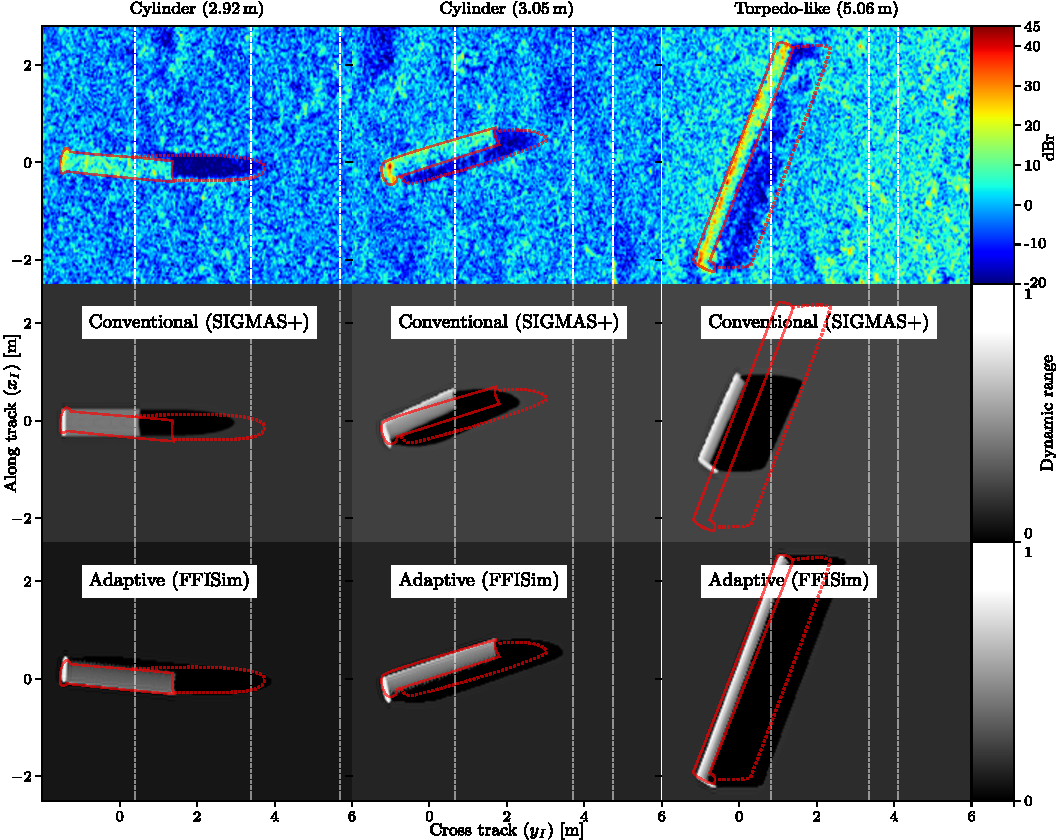
\includegraphics[width=1.25\linewidth]{gfx/fig_images_sonar_simulator_tagged.pdf}}%
\else
\begin{figure*}[t]\centering%
\ifOverLeaf%
  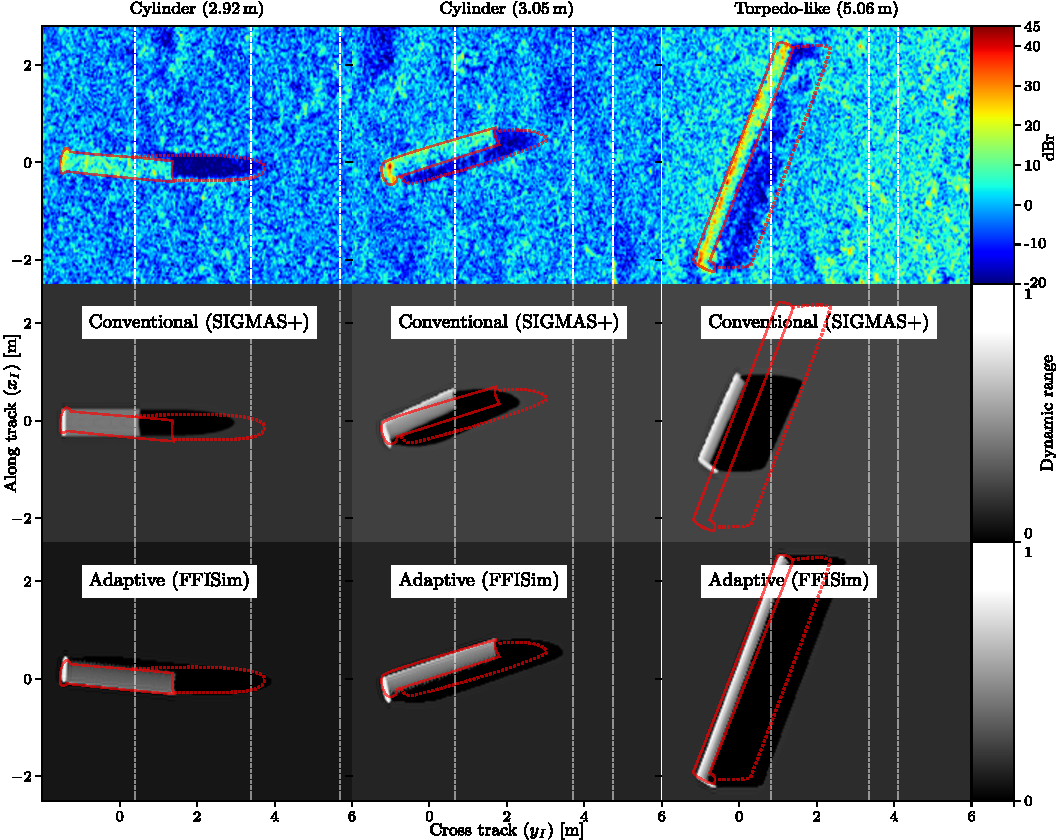
\includegraphics[width=.8\linewidth]{gfx/fig_images_sonar_simulator_tagged.pdf}%
\else%
  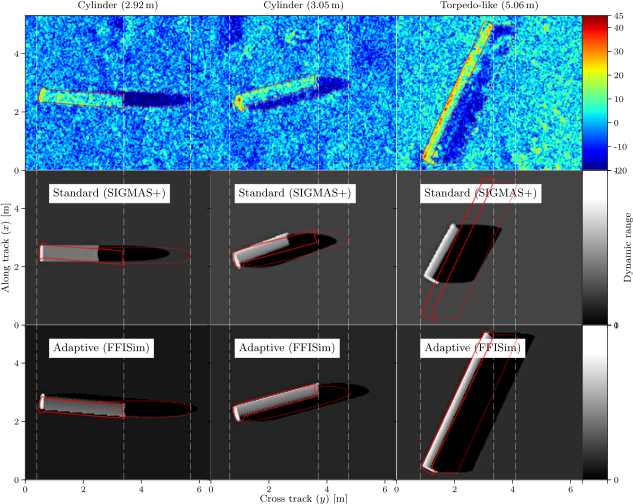
\includegraphics[width=.8\linewidth]{gfx/fig_images_sonar_simulator_tagged.svg}%
\fi\fi
\caption{\emph{Two cylinders and a torpedo in Jesus Bay, Norway.} Top row shows isolated SAS image segment corresponding to the object, while center and bottom rows show the template from the conventional and adaptive method, respectively. The contour of the SAS object is indicated with red lines. Observe that the adaptive technique performs better in highlight but not necessarily in shadow.}\label{IV_fig_images_sonar_simulation}%
\end{figure*}

\begin{figure*}[t]\centering%
\ifPhdDoc
  \vspace{-1cm}
  \makebox[\linewidth][c]{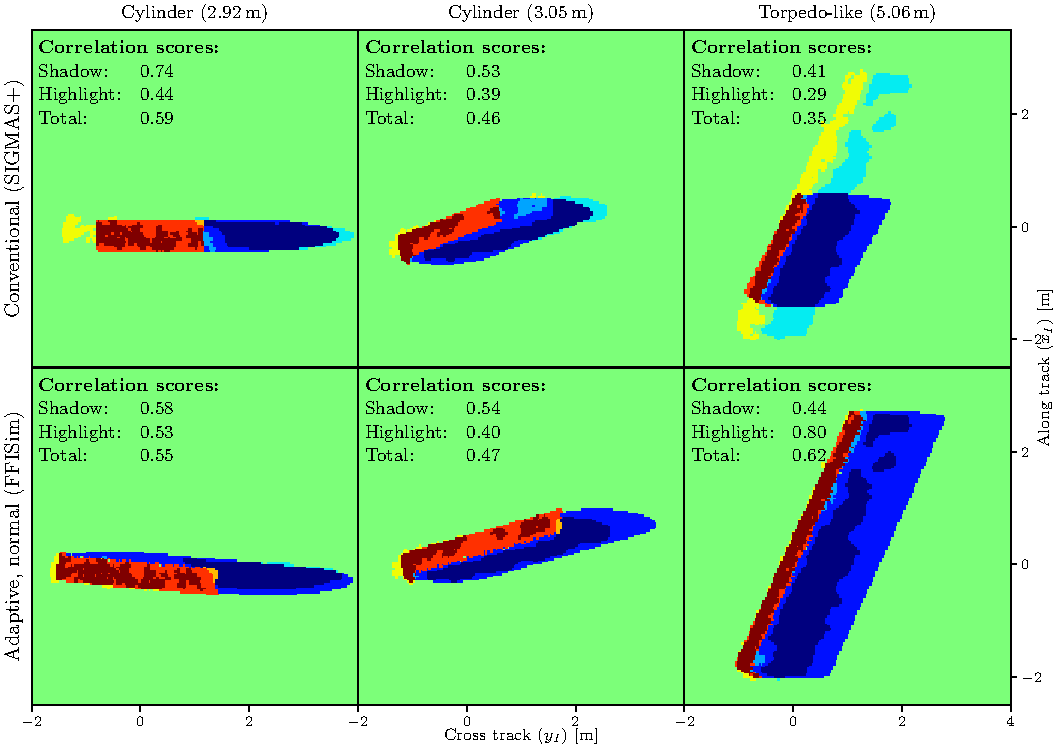
\includegraphics[width=1.25\linewidth]{gfx/fig_overlay.pdf}}
\else
   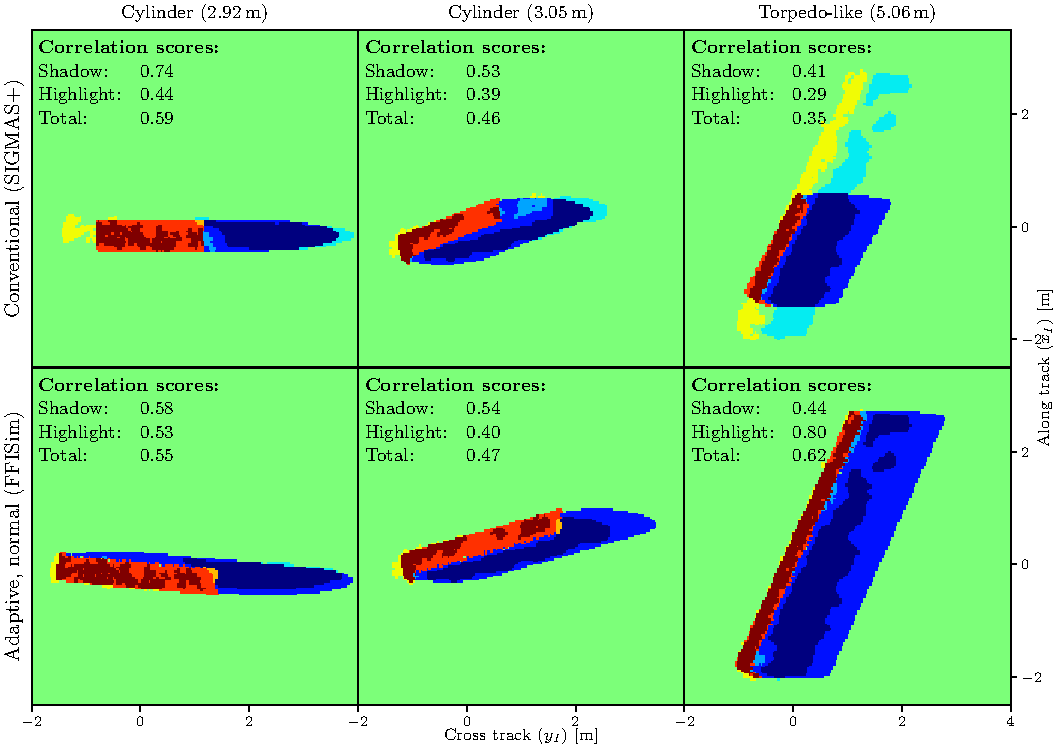
\includegraphics[width=\linewidth]{gfx/fig_overlay.pdf}
\fi%
% \parbox{\linewidth}{\small\centering\vspace{.5\baselineskip}
% \newline\centering\newline %\\[.5\baselineskip]
\newcommand\cdesc[2]{{\raggedright\setlength\fboxsep{0pt}
\fbox{\colorbox[HTML]{#1}{\vrule height8.5pt depth3.5pt width0pt\hspace{.5cm}}}\ \ #2\\}}
\begin{minipage}{.29\linewidth}\footnotesize
\cdesc{800000}{Template highlight and image highlight}
\cdesc{FF1000}{Template highlight only}
\cdesc{FFEB00}{Image highlight only}
\cdesc{83FF7C}{Background pixels}
\end{minipage}\mbox{}\hspace{3cm}
\begin{minipage}{.29\linewidth}\footnotesize
\cdesc{000083}{Template shadow and image shadow}
\cdesc{0014FF}{Template shadow only}
\cdesc{00EFFF}{Image shadow only}
\cdesc{00A7FF}{Template shadow and image highlight}
\end{minipage}%}
\caption[zzz]{Classification performance for the conventional and adaptive template techniques. Three objects were arbitrary picked from the scene. For two roughly 3\,m long cylinders the performance was similar or slightly in favor of the conventional method, which was expected since a 3\,m long cylindric model made up most of its static template database. However, for a longer torpedo-like object the adaptive technique was clearly better, which is its key merit: being able to adapt to uncommon objects not included in the static template database.}\label{IV_fig_image_simulation}%
\end{figure*}


\begin{figure*}[t]\centering%
\ifPhdDoc
\makebox[\linewidth][c]{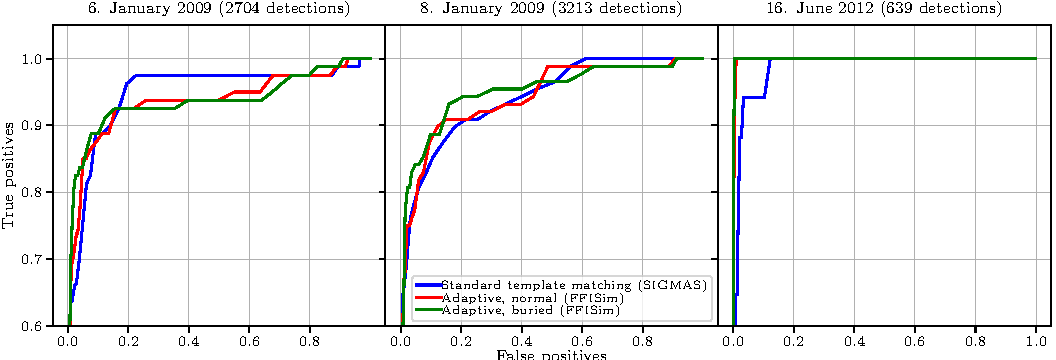
\includegraphics[width=1.25\linewidth]{gfx/fig_rocs.pdf}}
\else
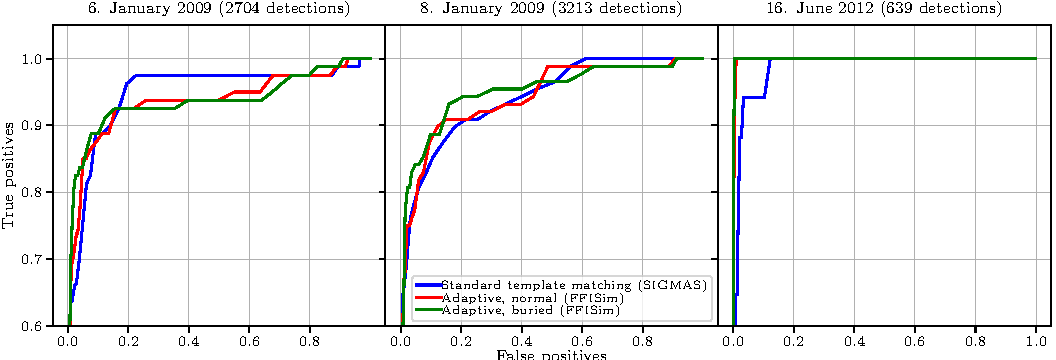
\includegraphics[width=\linewidth]{gfx/fig_rocs.pdf}%
\fi
\caption{\emph{Receiver operating characteristics (ROC) curves.} The adaptive methods outperform the conventional one below 20\% FRP, with additional adaption to burial depth increasing the advantage. Above 20\% FRP the methods tie. This suggests significant potential for improving performance in this scenario by increasing adaptivity.}\label{IV_fig_roc_curves}%
\end{figure*}

Our results are based on experimental data from a HISAS1030 interferometric synthetic aperture sonar (SAS) attached to a HUGIN autonomous underwater vehicle (AUV), both developed by Kongsberg Maritime, Norway. The HISAS1030 is a fully digital phased array with 32 hydrophones, 100\,kHz center frequency, 30\,kHz bandwidth, 1.2\,m length, 23$^\circ$ half-power beamwidth (HPBW) and 3-4\,cm theoretical resolution both cross- and along-track. Our version of HUGIN also carries a camera that is used for optical inspection of interesting objects.

%To test performance of our simulator and template matching techniques where measured using experimental data from 

We present three different HUGIN runs from Jesus Bay in Norway. The first pair of runs were two days apart in January 2009, containing roughly 2700 and 3200 detections, respectively. The last was in June 2012, containing roughly 650 detections. Almost all objects here are cylindric---e.g. barrels, pipe mines and torpedoes---with a length of about 3\,m.

For each run we contrast three template methods:
%
\begin{itemize}
\item \emph{Conventional (SIGMAS+).} Picks the best template from a set precomputed with SIGMAS+. The templates are tailored to a 3\,m long cylinder; the most frequently occurring object in the scene.
\item \emph{Adaptive, normal (FFISim).} Creates a single template with FFISim, given estimated seafloor and object orientation, and object length, width and immersion depth~\cite{Midelfart2010}. 
\item \emph{Adaptive, buried (FFISim).} Finds an "optimal" template with FFISim, given the estimated parameters described above and a search space for burial depth---modeled as rotation by $\{-4,-2,0,2,4\}^\circ$ around $\hat{y}_{I}$.
\end{itemize}

\subsection{Processing speed}


%The key selling point of FFISim is that it is very fast.  tighter integration with the classifier
%
%is used with the adaptive method due to its tighter integration with the classifier, allowing a range of templates to be generated and assessed on the GPU in a single invocation. It can produce thousands of templates per second if need be. This is why FFISim is being used in the adaptive procedure, and SIGMAS+ in the conventional procedure with a static precomputed set of templates.


Our simulator computes thousands of one-megapixel templates per second on a computer with six-core Intel Core i7-3930K CPU and Radeon HD7970 GPU. It achieves this with minimal memory footprint, full model search space and flexible post-processing, unlike the conventional method. This lays the groundwork for an entirely GPU-based template matcher and classifier with unrivaled real-time adaptivity.



\subsection{Classification - selected objects}

We contrast simulation and classification performance on three typical objects from the 2012 data: two roughly 3\,m long mines and a 5\,m long torpedo, each with unique immersion depths and aspect angles. SAS image segments and templates for these objects are shown in \Fig{IV_fig_images_sonar_simulation}, with hand-drawn red lines superimposed to reference the objects' contours. Observe the following:
%
\begin{itemize}
\item \emph{Template image quality} is similar for both SIGMAS+ and FFISim. With accurate input parameters, both simulators generate highlight and shadow regions with correct size and shape. Intensity values are also nearly identical (ignoring background level), as expected since both rely on a Lambertian scattering model.
\item \emph{Template accuracy} improves when using the adaptive technique; it excels at generating accurate highlight regions, but is less convincing in shadow regions. The less common the object, the poorer its representation by the static database, the greater the advantage of the adaptive method.
\end{itemize}

\ifPhdDoc
\FloatBarrier
\fi

\subsection{Classification - all objects}

Classification performance on all objects is demonstrated with receiver operating characteristic (ROC) curves in \Fig{IV_fig_roc_curves}. They illustrate the classification trade off between true positive rate (TPR) and false positive rate (FPR)---also called sensitivity and (inverse) specificity, or hit rate and alarm rate---as a function of different threshold values. A skillful model assigns higher probability to a positive occurrence than a negative one. Perfect skill is represented at the point $(0,1)$ and no skill at $(0.5,0.5)$. Observe the following:
%
\begin{itemize}
\item \emph{Below 20\% FPR} the adaptive techniques outperformed the static method in every run. This benefits e.g. mine counter measures (MCM) operations where only a few detections out of 3000 will be visually inspected up close.
\item \emph{Above 20\% FPR} the results are less clear: the adaptive techniques performed similarly to the static method in 2012, worse 6 January 2009 and better 8 January 2009---with 5 and 3 false detections at 20\% FPR, respectively. From visual inspection we found the cause to be a combination of fish trawler tracks and poor highlight and shadow quality.
\end{itemize}
%
A classification model should be neither too simple (high bias or underfitted) nor complex (high variance or underfit), but strike a balance between the two that captures statistically significant details of the object but not the noise. Higher detail-to-noise ratios favor more complex models and occur at lower FRP, where poor quality objects are discarded. The added complexity of the adaptive techniques seems beneficial here, yielding greater advantage at higher detail levels without suffering at lower ones. The greatest edge is held by the adaptive technique that also adjusts burial depth. The results suggest significant potential for improving performance by raising adaptivity in this scenario.


%
%The greater the detail, the greater potential advantage of adaptive algorithms.


% Concetional too simple
% Higer noise similar
% Higher true positives better performance
% yields greater advantage to the adaptive methods


% Bias vs variance
% High noise high variance
% Too simple model high bias
% Too complex model adapts to noise
%
% High variance, overfitting, adaptive method more susceptible
% High bias, underfitting, conventional method more susceptible
% Best performance at the ideal compromize between the two.


\section{Conclusion}\label{IV_conclusion}

Classification accuracy of adaptive template matching improves relative to conventional static methods with:
%
\begin{itemize}
\item \textit{On-the-fly simulation}, adapting better to the scenario at hand;
\item \textit{Faster processing speed}, paving the way for better adaptivity and real-time applications;
\item \textit{Increased flexibility}, allowing alternative simulation strategies for uncommon scenarios;
\item \textit{Improved image quality}, because adaptive methods yield a better advantage the more detailed the scene; 
\item \textit{Lowered false positive rate}, as it discards low quality objects.
\end{itemize}

The simulator was described with a rigorous and unified navigational notation system from K. Gade, which we adapt to computer graphics by extending its:
%
\begin{itemize}
\item \emph{Free form}---that promotes geometrical reasoning, conceptual insight and physical understanding---with \emph{topological ideas} from robotics and an abstraction level raised to that of \emph{affine transformations}, and 
\item \emph{Decomposed form}---that ensures geometrical validity and clarity when handling coordinates---with \emph{homogeneous coordinates} for affine transformations and usage ideas for arbitrary functions.
\end{itemize}

%We abide by a notation system with a:
%%
%\begin{itemize}
%\item \emph{Free form} promoting geometrical reasoning, conceptual clarity and physical clarity, a
%\item \emph{Decomposed form} ensuring geometrical validity and clarity when constructing, manipulating and interpreting coordinates, and a
%\end{itemize}
%
%\item \emph{Unified way} of expressing transformations in terms of
%\begin{itemize}
%\item positions denoted $\udot{P}$
%\item orientation, denoted $\uvec{V}$, governed by
%\end{itemize}
%\item subscripts governed by 
%\item transformation through multiplication of homogeneous matrices, under the constraint of identical composition and closest frame,
%\item translation through addition of vectors, under the constraint of identical decomposition and closest frame,
%\item rotation through multiplication of rotation matrices, under the constraint of identical decomposition and closest frame,
%\item vectors must be identically decomposed under addition,
%\item rotation matrices 
%\item nearest frame cancellation.
%\end{itemize}
%
%
%
%The notation system used to describe the simulator has a:
%%
%\emph{Free form} promoting geometrical reasoning, conceptual insight and physical understanding, a
%\emph{Decomposed form} ensuring geometrical validity and clarity when constructing, manipulating and interpreting coordinates, and a
%\emph{Unified way} of expressing transformations in terms of positions and orientations.
%% 
%We extended this 
%and extended 
%
%\begin{itemize}
%\item positions denoted $\udot{P}$
%\item orientation, denoted $\uvec{V}$, governed by
%\end{itemize}
%\item subscripts governed by 
%\item transformation through multiplication of homogeneous matrices, under the constraint of identical composition and closest frame,
%\item translation through addition of vectors, under the constraint of identical decomposition and closest frame,
%\item rotation through multiplication of rotation matrices, under the constraint of identical decomposition and closest frame,
%\item vectors must be identically decomposed under addition,
%\item rotation matrices 
%\item nearest frame cancellation.
%\end{itemize}



% However, when this was not the case, it was less clear who the winner was. The conventional method of using a static template library generally did well here.\todo{Meh. Fix fix fix}

% Template quality was similar with both SIGMAS+ and FFISim. The main difference lies in how they integrate into the classification process: SIGMAS+ generates one template for each invocation, FFISim iterates through a space of parameters on the GPU before returning control to the CPU. This speeds up the template matching dramatically, allowing it to assess thousands of templates per second instead of, say, one. \todo{lol, I will}
 
%
%\begin{itemize}
%\item Motion compensation
%\item 
%\end{itemize}

\ifPhdDoc
%\clearpage
\appendix
\renewcommand\thesection{\Alph{section}}
\renewcommand\thesubsection{\Alph{section}.\arabic{subsection}}
\else
\appendices
\fi

\section{Euler-Rodrigues rotations}\label{IV_sec_transformation_matrices}

Rotations are special linear operations with many possible free and decomposed formulations. A common one is Euler-Rodrigues formula, an axis-angle representation introduced by Euler in 1775 with many modern developments~\cite{Dai2015}. % in e.g. the study of coordinate free geometry, quaternions and Lie algebra.
%It parametrizes the rotation in terms of a half-angle  


\subsection{Free notation}\label{IV_sec:euler_rodrigues_free}

Euler-Rodrigues formula rotates a vector $\vec{p}$ by angle $\theta$ clockwise around unit-vector $\hat{r}$ in $\mathbb{R}^3$ Euclidean space,
%
\begin{align}\label{IV_eq_euler_rodrigues_free}
\vec{p}_\mathrm{rot} =  \vec{p} + 2a(\vec{\omega}\times\vec{p}) + 2(\vec\omega \times (\vec\omega \times \vec{p}))
\end{align}
%
where $\times$ denotes cross product, and
%
\begin{align}\label{IV_eq_euler_rodrigues_parameters}
a = \cos\frac{\theta}{2} \quad \text{and} \quad
\vec\omega = \hat{r}\sin\frac{\theta}{2}
\end{align}
%
are Euler-Rodrigues axis-angle parameters. Substituting these into \eq{IV_eq_euler_rodrigues_free} and recognizing the trigonometric identities $\sin^2\theta = \frac{1}{2}(1-\cos2\theta)$ and $\cos\theta\sin\theta=\frac{1}{2}\sin2\theta$ yields the alternative form
%
\begin{align}
\vec{p}_\mathrm{rot} =  \vec{p} + \sin\theta(\hat{r}\times\vec{p}) + (1-\cos\theta)(\hat{r} \times (\hat{r} \times \vec{p})),
\end{align}
%
where $\hat{r}$ and $\theta$ are Euler axis-angle parameters. Factoring out $\vec{p}$ from this equation yields a \emph{rotation dyadic} $\vec{R}$,
%
\begin{align}
\vec{R}_{\mathrm{er}}(\hat{r},\theta) =  \vec{I} + \sin\theta{}S(\hat{r}) + (1-\cos\theta)S^2(\hat{r}),
\end{align}
%
where $\vec{I}$ is an identity dyadic and $S(\hat{r}) = [\hat{r}\times]$ is the skew-symmetric dyadic form of $\hat{r}$. Dyadics are tensors of rank 2 with a vector-like notation. They resemble matrices but are basis-vector independent, ideal for free notation. 

We denote a rotation $\uvec{A}\to\uvec{B}$ with subscripts: $\vec{R}_{\mathrm{er},AB}$, $\hat{r}_{AB}$ and $\theta_{AB}$.

\subsection{Decomposed notation}\label{IV_sec:euler_rodrigues_decomposed}

Euler-Rodrigues' formula adopts a very similar decomposed form,
%
\begin{align}
\mat{R}_{\mathrm{er}}
&= \I + \sin\theta{}\mat{S}(\dhat{r}) + (1-\cos\theta)\mat{S}^2(\dhat{r})\label{IV_eq_euler_rodrigues_decomposed} \\
&= e^{\theta{}\mat{S}(\dhat{r})} \in\mathrm{SO}(3)\label{IV_eq_euler_rodrigues_exponential},
\end{align}
%
where $\theta\in[0,\pi]$ and $\mat{S}(\dhat{r})$ denotes the skew-symmetric matrix form of $\dhat{r}\in\mathbb{R}^3$,
%
\begin{align}
\mat{S}
&= \bmat{
0 & -\hat{r}_z & \hat{r}_y \\
\hat{r}_z & 0 & -\hat{r}_x \\
-\hat{r}_y & \hat{r}_x & 0
} \in\mathfrak{so}(3).
\end{align}
%
The equality between the matrix trigonometric\todo{Correct?} in \eq{IV_eq_euler_rodrigues_decomposed} and the matrix exponential in \eq{IV_eq_euler_rodrigues_exponential} may be verified by Taylor expansion about $\theta=0$. Note how axis-angle parameters are related to rotation matrices by the exponential function. Stated in group theory terms: possible rotations make up the Lie group $\mathrm{SO}(3)$, possible axis-angle pair make up the Lie algebra $\mathfrak{so}(3)$, and an exponential map relates them.

% The action of rotation can be represented by the Lie group SO3 under multiplication, or by the Lie algebra so3 under addition, 

% Group - collection of symmetric actions?
% 
% Ordinary exponential function: Special case of the exponential map when G is the multiplicative (symmetry) group of postive real numbers, whose Lie algebra is the additive group of real numbers.

% Action associated with 


% continuous domain (no discontinuties) = differentiable
% SO(3) is diffeomorphic ({N,M} in SO(3), differentiable f: M to N is bijective and has differentible inverse) to the real projective space RP3

% diffeomorphic (both differentiable, bijective map): so(3) -> SO(3), SO(3) -> RP3
% homomorphic   ( f(X Y) = f(X) f(Y) (same shape)
% homeomorphic  (continuous map, continuous inverse) 
% isomorphic:    so(3) -> su(2)
% (same as homomorphic?)
%
% homoemorphisms are usually diffeomorphic (exceptions found in 4 or more dimensions)
% 
% actions 

% - A group is a collection of symmetrical actions on some mathematical object.
% - Every group has a certain arthmetic, where one can combine two actions by applying one after the other and asking: what other action from the group gives the same overall effect?
% - Number can be thought of in two different ways as a group
%   1. Act by sliding actions 	                   (group arithmetic looks like addition)
%   2. Act by stretching/squishing/rotating actions (group arithmetic looks like multiplication)
% Group of actions on a set of mathematical objects
% Action associated with mathematical object(s).
% Group of symmetrical sliding actions
% Group of symmetrical stretching/squishing actions
% Groups of symmetries acting on some object

\section{Quaternion rotations}\label{IV_sec_quaternions}

Quaternions are a popular alternative to rotation matrices in computer graphics. They represent orientation by the four Euler-Rodrigues parameters in \eq{IV_eq_euler_rodrigues_parameters},
%
\begin{align}\label{IV_eq_quaternion}
\dvec{q} = \bmat{a & \boldsymbol\omega} = \bmat{\cos\frac{\theta}{2} & \dvec\omega^T\sin\frac{\theta}{2}} \in\mathbb{R}^4
\end{align}
% 
subject to $\rVert \dvec{q} \rVert = 1$. Unit length quaternions are called versors and have their own Lie group\todo{details. bijective?}. We denote a rotation $\uvec{A}\to\uvec{B}$ as $\dvec{q} = \dvec{q}_{AB}(\theta_{AB},\dhat{r}_{AB}^A)$ and apply it with 
%
\begin{align}\label{IV_eq_quaternion_usage}
\dvec{p}^{\v{A}} = \dvec{q}\dvec{p}^{\v{B}}\dvec{q}^*,
\end{align}
%
where $\dvec{q}^*$ negates the three last coefficients ($\dvec\omega$). To use our notation system, we wrap \eq{IV_eq_quaternion_usage} into a function $\mathrm{T}_{\mathrm{qu}}$,
%
\begin{align}\label{IV_eq_quaternion_function}
\nonumber\\
\dvec{p}^{\,\v[R1]{A}}
= \mathrm{T}_{\mathrm{qu},\v[R2]{A}\c[C1]{B}}(\dvec{p}^{\c[C2]{B}}).
%
\tikz[overlay,remember picture]{
  % Set up some general bounding box markers
%  \coordinate(_MV)  at ($   (V.south)    + (-1.0\baselineskip,-1.0\baselineskip) $);
  \coordinate(_R1)  at ($ (R1.north) + ( 1.0\baselineskip,1.0\baselineskip) $);
  \path let \p1 = ($ (R2.north) + (-1.0\baselineskip,0ex) $), \p2 = (_R1) in coordinate (_R2)  at (\x1,\y2);
%   \coordinate(_I3)  at ($ (I3.north) + (-1.0\baselineskip,1.0\baselineskip) $);
  \coordinate(_R12)  at ($ .5*(_R1) + .5*(_R2) $);
  % Draw arrows and text
%           to[out=180, in=0]    (_I1)
    \draw[color=cDarkArrow]      ($ (R2.north) + (0em,\tpad) $)
           to[out=90,  in=0]    (_R2)
           to[out=180, in=0]    (_R1)
           to[out=180, in=90]($ (R1.north) + (0em,\tpad) $);
    }
\end{align}
%
Quaternions can reduce computational complexity, improve numerical stability and facilitate efficient spherical interpolations compared to rotation matrices, but lack the nice formal properties of the latter. 


%(Quaternions: 4 parameters = 3 user-defined degrees of freedom + 1 constraint (unit length). Called versor. Is a Lie group. Not bijective(?))



%Another convenient, non-singular and practical alternative is the $\vec n$-vector notation~\cite{Gade2010}. 

%
%(TODO: Elaborate on robotics advantage of using matrix exponential)
%
%(TODO: Quaternions, simply insert the Euler-Rodrigues parameters)

%
%G = exp(g)
%
%G - multiplicative group of positive real numbers
%g - additive group of all real numbers
%
%SO(3) - the multiplicative group of proper rotations
%so(3) - the additive group of 




%%
%and the angle $\theta$ and rotation axis $\hat{r}_{AB}$ can be expressed in terms of $\vec{p}_A$ and $\vec{p}_{B}$,
%%
%\begin{align}
%\theta
%&= \mathrm{acos}\frac{\vec{p}_{A}\cdot\vec{p}_{B}}{\lVert\vec{p}_{A}\rVert\lVert\vec{p}_{B}\rVert} \\
%\hat{r}_{AB} &=  \frac{\vec{p}_{A}\times\vec{p}_{B}}{\lVert\vec{p}_{A}\rVert\lVert\vec{p}_{B}\rVert}
%\end{align}
%%
%where $\cdot$ and $\times$ denotes the dot- and cross-product, respectively.


%~\cite{Murray1994}\footnote{Pages 26-27}\todo{Valid page specification?}.

%The rotations are performed with Euler-Rodrigues formula~\cite{Dai2015} using a unit length rotation axis $\dvec{\hat{r}}_{AB}^A$ and angle $\theta_{AB}$:
%%
%%
%where $\big[\dvec{\hat{r}}_{AB}^A\big]$ is the open-right cross product matrix of $\dvec{\hat{r}}^A$ and $\mat{I}$ is the identity matrix. 
%
%% %\dvec{\hat{p}}_{A\times{}B}^C
%\begin{align}
%\theta_{AB}
%&= \mathrm{acos}\frac{\dvec{p}_{A}^{C}\cdot\dvec{p}_{B}^{C}}{\lVert\dvec{p}_{A}^{C}\rVert\lVert\dvec{p}_{A}^{C}\rVert} \\
%\dvec{\hat{r}}_{AB}^C &=  \frac{\dvec{p}_{A}^{C}\times\dvec{p}_{B}^{C}}{\lVert\dvec{p}_{A}^{C}\rVert\lVert\dvec{p}_{A}^{C}\rVert}
%\end{align}

\section{Euler rotations}\label{IV_sec_euler_angles}

End-users often prefer Euler or Tait-Brian angles over axis-angle parametrizations. They specify an orientation composed from three elementary rotations; Euler rotations about the same first and third axis, or Tait-Brian rotations about three unique axes. The rotations can either be intrinsic or extrinsic, depending on whether the coordinate system follows the rotation or stays fixed, respectively. We use the intrinsic Tait-Brian $Z$-$Y'$-$X''$ convention, with the \emph{nautical angles} yaw ($\phi$), pitch ($\theta$) and roll ($\psi$), representing clockwise rotations around the intrinsic $z$-, $y$- and $x$-axis, respectively. In this convention, roll is applied first, then pitch and finally yaw,
%
\begin{align}
\R_{\mathrm{eu}} = \R_z(\phi)\R_y(\theta)\R_x(\psi),
\end{align}
%
where
%
\begin{align}
\R_x(\psi) &= \bmat{
    1  &   0        &  0         \\
    0  &  \cos\psi  &  -\sin\psi \\
    0  &  \sin\psi  &  \cos\psi 
}, \\[.5\baselineskip]
\R_y(\theta) & = \bmat{
\cos\theta	& 0          & \sin\theta \\
0				& 1          & 0          \\
-\sin\theta & 0          & \cos\theta 
},
%\\[0\baselineskip]
\intertext{and}
%\\[0\baselineskip]
\R_z(\phi) &= \bmat{
\cos\phi	&  -\sin\phi   &  0       \\
\sin\phi	&  \cos\phi    &  0       \\
0			&  0           &  1       
}.
\end{align}
%
At $\theta=\frac{\pi}{2}$ we have $\phi=-\psi$, and at $\theta=-\frac{\pi}{2}$ we have $\phi=\psi$. This effect, in which one degree of freedom is lost, is known as Gimbal lock. Any three-parameter specification of an orientation in three-dimensional space has this problem. Axis-angle representations such as Euler-Rodrigues formula or quaternions avoids this issue by adding a fourth parameter and one constraint: one angle and three parameters for the rotation axis subject to unit length. 



\section{Active vs. passive rotations}\label{IV_sec:active_passive_rotations} 

The geometrical intent of an active rotation is to move a point, by contrast the passive version instead changes the point's representation. With our notation this can be expressed as either
%
\begin{align}
\m{CL}
\vec{p}_{M\d[Vtot]{V}_{\color{cBaseMark}\!\textrm{new}}}
= \vec{R} \; \vec{p}_{M\d[V2]{V}}\m{CR}
\quad\text{or}\quad
\m{CL2}
\dvec{p}_{M\d[Vtot2]{V}_{\color{cBaseMark}\!\textrm{new}}}^M
= \mat{R}^M \dvec{p}_{M\d[V4]{V}}^M,\m{CR2}
\label{IV_eq_active_rotation}
 \\\nonumber
 %\qquad\qquad
%
%\\[.5\baselineskip]\nonumber % Adjust spacing as necessary
\tikz[overlay,remember picture]{
  % Set up some general bounding box markers
  \coordinate(CC) at      ($ .5*(CL)       + .5*(CR)                         $);
  \coordinate(CC2) at     ($ .5*(CL2)      + .5*(CR2)                        $);
  \coordinate(_MV) at     ($ (V2.south)    + (-\baselineskip,-\baselineskip) $);
  \coordinate(_MVtot) at  ($ (Vtot.south)  + ( \baselineskip,-\baselineskip) $);
  \coordinate(_MV2) at    ($ (V4.south)    + (-\baselineskip,-\baselineskip) $);
  \coordinate(_MVtot2) at ($ (Vtot2.south) + ( \baselineskip,-\baselineskip) $);
  % Draw arrows and text
    \draw[]                    ($ (V2.south)    - (0em,\tpad) $)
            to[out=-90, in=0]     (_MV)
            to[out=180, in=0]     (_MVtot)
            to[out=180, in=-90]($ (Vtot.south)  - (0em,\tpad) $);
    \draw[]                    ($ (V4.south)    - (0em,\tpad) $) 
            to[out=-90, in=0]     (_MV2)
            to[out=180, in=0]     (_MVtot2)
            to[out=180, in=-90]($ (Vtot2.south) - (0em,\tpad) $);
}
\end{align}
%
%
% Implicit representation: (x,y,z) subject to x²+y²+z²=c -> no 
depending on whether the free or decomposed form is wanted, and where $\vec{R}\colon \mathbb{V}^N \to \mathbb{V}^N$ and $\dvec{R}^M\colon \mathbb{R}^N \to \mathbb{R}^N$. Beware that the rotation matrix can be identical---both notationally and numerically---in the active and passive case, for example, if $\dvec{R}^M$ was replaced by $\dvec{R}_{IM}$ in \eq{IV_eq_active_rotation}. Thus, the geometrical intent must be inferred from the position vector notation; either the point changes, or the representation does, but never both.





% http://lairs.eng.buffalo.edu/pdffiles/pconf/C10.pdf
% http://www.navlab.net/Publications/Inertial_Navigation_-_Theory_and_Applications.pdf




%xyz - system space coordinates (fixed unmoving)
%XYZ - system body coordinates (body fixed moving)



%and the bases in terms of a linear operator $\vec{R}_{AB} \in SO(3)$ which rotates around an axis $\hat{r}$ by angle $\theta$,
%%
%\begin{align}\label{eq:M}
%\vec{R}_{AB}
%&=
%% \vec{I} + \overset{\times}{r}\sin\theta + \overset{\times}{r}{}^2(1-\cos\theta).
%\vec{I} + \sin\theta(\hat{r}\times) + (1-\cos\theta)(\hat{r}\times)^2.
%\end{align}
%%
%where $\times$ is the cross-product. $\hat{r}$ and $\theta$ relates to $\uvec{A}$ and $\uvec{B}$ by
%%
%\begin{align}
%\hat{r} = \frac{\uvec{A}\times\uvec{B}}{\lVert\uvec{A}\rVert\lVert\uvec{B}\rVert}
%\quad\mathrm{and}\quad
%\theta  = \mathrm{acos}\frac{\uvec{A}\cdot\uvec{B}}{\lVert\uvec{A}\rVert\lVert\uvec{B}\rVert},
%\end{align}
%%
%where $\times$ and $\cdot$ signifies the cross- and dot-product, respectively.
%
%and the angle $\theta$ and rotation axis $\hat{r}_{AB}$ can be expressed in terms of $\vec{p}_A$ and $\vec{p}_{B}$,
%%
%\begin{align}
%\theta
%&= \mathrm{acos}\frac{\vec{p}_{A}\cdot\vec{p}_{B}}{\lVert\vec{p}_{A}\rVert\lVert\vec{p}_{B}\rVert} \\
%\hat{r}_{AB} &=  \frac{\vec{p}_{A}\times\vec{p}_{B}}{\lVert\vec{p}_{A}\rVert\lVert\vec{p}_{B}\rVert}
%\end{align}
%\begin{align}
%\theta
%&= \mathrm{acos}\frac{\vec{p}_{A}\cdot\vec{p}_{B}}{\lVert\vec{p}_{A}\rVert\lVert\vec{p}_{B}\rVert} \\
%\hat{r}_{AB} &=  \frac{\vec{p}_{A}\times\vec{p}_{B}}{\lVert\vec{p}_{A}\rVert\lVert\vec{p}_{B}\rVert}
%\end{align}
%%
%The position vector $\vec{p}_{\udot{A}\udot{B}}$ go from $\udot{A}$ to $\udot{B}$ only depends on these points. Similarly, the matrix $\vec{R}_{\uvec{A}\uvec{B}}$ only depends on vectors; $\vec{R}_{\uvec{A}\uvec{B}}\uvec{B}$ rotates $\uvec{B}$ to $\uvec{B}$, $\uvec{A}\vec{R}_{\uvec{A}\uvec{B}}$ rotates $\uvec{A}$ to $\uvec{B}$. 
%


% use section* for acknowledgement
\ifCLASSOPTIONcompsoc% % This command fixes abstract positioning for compsoc articles:
% \IEEEdisplaynotcompsoctitleabstractindextext
% 
% % (Optional) Add some extra info on cover page of peer review papers:
% % \ifCLASSOPTIONpeerreview
% % \begin{center} \bfseries EDICS Category: 3-BBND \end{center}
% % \fi
% 
% % Insert page break and insert second title (peer review mode)
% \IEEEpeerreviewmaketitle
% 
% 
% 
  \section*{Acknowledgments}
\else
  \section*{Acknowledgment}
\fi


The authors would like to express their gratitude to the Norwegian Defence Research Establishment (FFI) for funding development of the simulator.

% Can use something like this to put references on a page
% by themselves when using endfloat and the captionsoff option.
\ifCLASSOPTIONcaptionsoff
  \newpage
\fi


\ifPhdDoc
   \printbibliography[title=References,heading=subbibliography]
   \addcontentsline{toc}{section}{References}
%    \bibliographysty
%    \bibliography{library.bib}
%    \print
\else
   \ifBuildBibliography
      \typeout{===Mybib===}
      \bibliographystyle{IEEEtran}
      \bibliography{references}

   \else
      \typeout{===MyStaticbib===}
      % Paste here
   \fi

  
   % Generated by IEEEtran.bst, version: 1.13 (2008/09/30)
   % \begin{thebibliography}{10}
   % stuff here
   % \end{thebibliography}
   
   
   
\begin{IEEEbiography}[{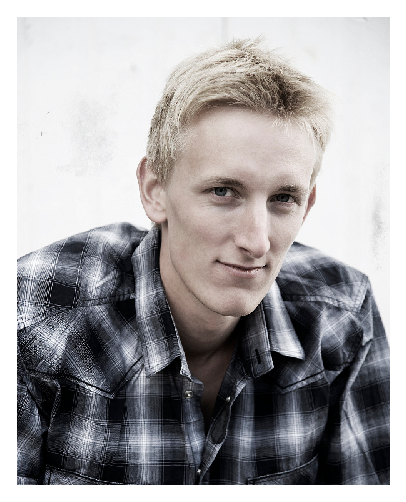
\includegraphics[width=1in,height=1.25in,clip,keepaspectratio]{bio/jo_inge.eps}}]{Jo Inge Buskenes}
received the B.Sc. degree in electrical engineering from Gj\o{}vik College University, Norway, in 2007, and the M.Sc. degree in instrumentation for particle physics from the University of Oslo, Norway, in 2010. He is currently pursuing the Ph.D. degree in acoustic image reconstruction and high performance computing at the University of Oslo.

His industry experience includes development of digital electronics at the European Organization for Nuclear Research (CERN), Geneva, Switzerland (2007-2008). He has lectured in digital signal processing at the Gj\o{}vik College University (2009), and at the University of Oslo (2010-2013). Current affiliation is with The Norwegian Defence Research Establishment, Kjeller, Norway, for which he is developing radar systems (2015-), and formerly sonar systems (2009, 2013).

His research interests include radar and sonar technology, aptive image reconstruction, high performance computing, intelligent detector design and open source software.
\end{IEEEbiography}
   
\begin{IEEEbiography}[{\includegraphics[width=1in,height=1.25in,clip,keepaspectratio]{bio/herman.eps}}]{Herman Midelfart}
held a M.Sc. and Ph.D. degree (2003) in genomics from the Norwegian University of Science and Technology (NTNU), Norway. Since 2007 he advanced research on automatic target recognition (ATR) in synthetic aperture sonar (SAS) at the Norwegian Defence Research Establishment, Kjeller, Norway.

Herman passed away in 2015. This work was finalized in his memory.
\end{IEEEbiography}

   % 
\begin{IEEEbiography}[{\includegraphics[width=1in,height=1.25in,clip,keepaspectratio]{bio/jon_petter.eps}}]{Jon Petter \AA{}sen}
(S'12) was born in Porsgrunn, Norway in 1986. He received the B.Sc. and M.Sc. degree in computer science from the University of Oslo, Norway, in 2010. He is currently pursuing his Ph.D. degree in medical ultrasound technology at the Norwegian University of Science and Technology (NTNU) Medical Imaging Lab (MI-Lab), Trondheim, Norway. His research interests include adaptive ultrasound processing techniques and acceleration of ultrasound algorithms using Graphics Processing Units (GPUs). 
\end{IEEEbiography}
   % 
\begin{IEEEbiography}[{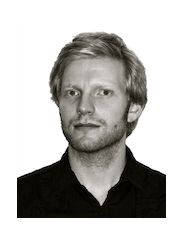
\includegraphics[width=1in,height=1.25in,clip,keepaspectratio]{bio/carl-inge.eps}}]{Carl-Inge Colombo Nilsen}
(S'06-M'10) received the M.Sc. and Ph.d. degrees in computer science from the University of Oslo, Norway, in 2005 and 2010. He is currently working at the University of Oslo as a postdoctoral research fellow. His research interests include signal and array processing for ultrasound imaging and other acoustical applications.
\end{IEEEbiography}
   % 
\begin{IEEEbiography}[{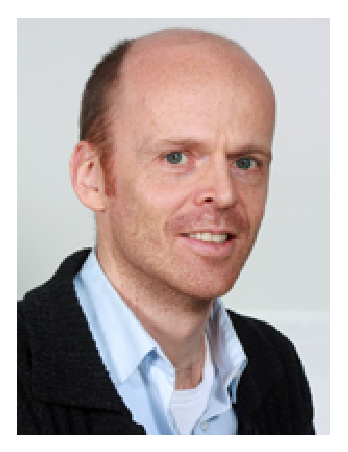
\includegraphics[width=1in,height=1.25in,clip,keepaspectratio]{bio/andreas.eps}}]{Andreas Austeng}
was born in Oslo, Norway, in 1970. He received the M.Sc. degree in physics in 1996 and the Ph.D. degree in computer science in 2001, both from the University of Oslo. Since 2001, he has been working at the Department of Informatics, University of Oslo, first as a postdoctoral research fellow and currently as an associate professor. His research interests include signal and array processing for acoustical imaging.
\end{IEEEbiography}
   
   
   % 
   % IMAGE METRICS
   %
   % - Point spread function (res via main lobe width, SAS gain via PDF height)
   % - Constrast measures
   %
   % ACR = cL/2
   % C = (s+n)/n ratio
   % - 
   % WHO's needing processing power
   % - Centre for Maritime Research and Experimentation
   
%   
%   \vfill 
%   
%   
\newpage

\section{Wave Equation}

The wave equation describes how a wave moves as a function of both time and space. It forms the basis for all mathematical modeling of waves, so we will spend some time to derive it here. We will treat acoustical waves since they are most relevant to the topic in this thesis, but we could have derived it from electromagnetic waves using Maxwell's equations with some boundary conditions.

\begin{figure}[ht]
\begin{floatrow}

\floatbox{figure}[\linewidth][\FBheight][t]{%
\caption{Mass flow}}{%
\graphicsAI[drawing,width=.77\linewidth]{gfx/wave_equation_mass_flow.svg}}%

\floatbox{table}[\linewidth][\FBheight][t]{%
\caption{Symbol description}}{%
\begin{tabular}[c]{c c l}\hline
\rowcolor{tabBlue}\bf Symbol & \bf Unit & \bf Description \\\hline
$s$ & Pa = N/m$^2$ & Pressure \\
$\rho$ & kg/m$^3$ & Density \\
$S$ & Nm/K & Entropy \\
$\vec v$ & m/s & Mass velocity \\
$\dot{\boldsymbol{m}}$ & kg/s & Mass flow
\end{tabular}}

\end{floatrow}
\end{figure}


We begin by defining the net \textbf{mass flow} through a volumetric element $dV = dx\,dy\,dz$:
%
\begin{align}
\frac{\dot{\boldsymbol{m}}_\text{net}}{dV} = \ux\frac{\partial \rho\,\v}{\partial x} + \uy\frac{\partial \rho\,\v}{\partial y} + \uz\frac{\partial \rho\,\v}{\partial z} = \nabla \cdot (\rho\v).
\end{align}
%
The space and time dependence of the mass density $\rho = \rho(\p,t)$ and particle velocity $\v = \v(\p,t)$ is omitted here and in the following text for brevity. If the volume of the element is fixed a change in mass must equal a corresponding change in density. This is the law of \textbf{mass conservation}:
%
\begin{align}
\frac{\partial\rho}{\partial t} = -\nabla \cdot (\rho\v). \label{wave_eq_mass_conservation}
\end{align}
%
An additional constraint we may surely apply is the Euler's equation, a modification of Newton's second law the the total acceleration $a$ is is a function of both time and space:
%
\begin{align}
\frac{F}{dV} = \frac{m}{dV} a = \rho\Big(\frac{\partial\v}{\partial t} + \v\cdot\nabla\v\Big) = -\nabla s. \label{wave_eq_euler}
\end{align}
%
Next, an \textbf{equation of state} is needed to relate a change in density to a change in pressure. We assume our volume element to be isentropic, i.e. that the entropy is constant, or equivalently that total energy of the system is proportional to its temperature. This is true for any system that is reversible and adiabatic, i.e. that when no transfer of matter or heat occurs between the system and its surroundings. The pressure of the system then just depends on the mass density:
%
\begin{align}
s = s(\rho) \label{wave_eq_sound_pressure}
\end{align}

With this we have assumed the system to be \emph{loss-less}. In reality a passing sound wave will heat the fluid and add to the entropy, causing additional attenuation of the wave, but we will not be concerned with attenuation in this thesis.

\subsection{Linearization}

Equation (\ref{wave_eq_mass_conservation}), (\ref{wave_eq_euler}) and (\ref{wave_eq_sound_pressure}) are non-linear, but can be linearized by assuming each quantity to be a steady-state, time-independent value plus a fluctuation term:
%
\begin{align}
s = s_0 + s'  \qquad\qquad \rho = \rho_0 + \rho' \qquad\qquad \v = \v_0 + \v'
\end{align}
%
Taylor expanding (\ref{wave_eq_sound_pressure}) around zero yields:
%
\begin{align}
s(\rho) = s_0 + \frac{\partial s}{\partial\rho}(\rho-\rho_0) + \frac{1}{2}\frac{\partial^2 s}{\partial\rho^2}(\rho-\rho_0)^2 + \dots\label{wave_eq_sound_taylor_full}
\end{align}
%
Assuming a linear relationship between changes in pressure and volume the pressure perturbation term is simply:
%
\begin{align}
s' = \frac{\partial s}{\partial\rho}(\rho-\rho_0) = \frac{\partial s}{\partial\rho}\rho' = c^2\rho'. \label{wave_eq_sound_taylor_first}
\end{align}
%
When treating the Euler equation the same way we obtain:
%
\begin{align}
-\nabla (s_0 + s') &= (\rho_0 + \rho') \Big(\frac{\partial(\v_0 + \v')}{\partial t} + (\v_0 + \v')\cdot\nabla(\v_0 + \v')\Big) \nn
-\nabla s' &= (\rho_0 + \rho') \Big(\frac{\partial\v'}{\partial t} + \v'\cdot\nabla\v'\Big) \nn
\end{align}
%
When acceleration mainly depends on time, and the pressure fluctuations are relatively small,
%
\begin{align}
\frac{\partial\v'}{\partial t} >> \v'\cdot\nabla\v' \qquad\qquad\text{and}\qquad\qquad \rho_0 >> \rho',
\end{align}
%
then
%
\begin{align}
-\nabla s' &= \rho_0 \frac{\partial\v'}{\partial t}.
\end{align}
%
Finally, for the mass conservation we have:
%
\begin{align}
\frac{\partial(\rho_0 + \rho')}{\partial t} &= -\nabla \cdot \big((\rho_0 + \rho')(\v_0 + \v')\big)\nn
\frac{\partial\rho'}{\partial t} &= -\rho_0\nabla \cdot \v'. \label{wave_eq_mass_conservation2}
\end{align}
%
This assumes that the density is constant inside the volume element.

\begin{align}
\nabla\cdot(-\nabla s') &= \nabla\cdot\Big(\rho_0 \frac{\partial\v'}{\partial t}\Big) &
\frac{\partial}{\partial t}\frac{\partial\rho'}{\partial t} &= \frac{\partial}{\partial t}\Big(-\rho_0\nabla \cdot \v'\Big)\nn
-\nabla^2 s' &= \rho_0 \nabla\cdot\frac{\partial\v'}{\partial t} &
\frac{\partial^2\rho'}{\partial t^2} &= \frac{1}{c^2}\frac{\partial^2 s}{\partial t^2} = -\rho_0\nabla\cdot\frac{\partial \v'}{\partial t}
\end{align}
%
and we can now see that
%
\begin{align}
\nabla^2 s' - \frac{1}{c^2}\frac{\partial^2 s'}{\partial t^2} = 0.
\end{align}
%
This is called the homogeneous lossless wave equation, because there is no source term. The inhomogeneous equation can be obtained in a similar way, by altering the linearized continuity equation to:
%
\begin{align}
\frac{\partial\rho'}{\partial t} &= -\rho_0\nabla \cdot \v' - \rho_0f(\p,t). \label{wave_eq_mass_conservation_source}
\end{align}
%
where $\rho_0f(\p,t)$ is the rate of mass change (in $\left[\frac{\text{kg}}{\text{m}^3\text{s}}\right]$) caused by the source. Following the exact same procedure as before we obtain:
%
\begin{align}
\nabla^2 s' - \frac{1}{c^2}\frac{\partial^2 s'}{\partial t^2} = \rho_0\frac{\partial f(\p,t)}{\partial t}.
\end{align}
%

\section{Solution}

Instead of solving the wave equation directly, we will make a qualified guess that the solution takes the form of a complex exponential in both time and space. For rectangular coordinates this can be written as:
%
\begin{align}
s(\p,t) &= A\,e^{j(\omega t - \k\cdot\p)}
\end{align}
%
Inserting this into the wave equation yields:
%
\begin{align}
\nabla^2 s = \frac{\partial^2 s}{\partial x^2} + \frac{\partial^2 s}{\partial y^2} + \frac{\partial^2 s}{\partial z^2} &= \frac{1}{c^2}\frac{\partial^2 s}{\partial t^2} \nn
(-jk_x)^2 s + (-jk_y)^2 s + (-jk_z)^2 s &= \frac{(-j\omega)^2}{c^2} s \nn
k_x^2 + k_y^2 + k_z^2 &= |\k|^2 = \frac{\omega^2}{c^2} \\
|\k| &= \frac{\omega}{c}
\end{align}
%
Hence, whenever we can assume the spatial and temporal frequency to be related directly by the sound speed, $|\k| = \frac{\omega}{c}$, then this assuming a complex exponential should be fair.

\section{Absorption}

Our derivation of the wave equation assumed no loss of energy. In practice the wave's energy is abosorbed through viscous losses, heat conduction losses and intermolecular losses. These are strongly dependent on frequency. The wave equation can be adapted to account for absorption by assuming a complex sound speed, which will lead to a solution to the wave equation with a real exponential term. In this thesis we will not concern ourselves 

\section{Roughness}

For a plane monochromatic wave the Rayleigh roughness parameter is quantified by:
\begin{align}
\Delta\varphi = 2k\xi\cos\theta.
\end{align}
Here $\theta$ is the incidence angle, $k = \frac{2\pi}{\lambda}$ is the wavenumber of the incoming wave, $\xi$ is the distance from the scattering point to the mean surface plane, and $\Delta\varphi$ is the phase difference.

\begin{figure}[th]
\graphicsAI[drawing,width=\linewidth]{gfx/roughness.svg}
\end{figure}

To see how roughness affects the specular reflection we compute the mean reflected wave as
\begin{align}
<p> &= V\int\limits_{-\infty}^{\infty} e^{-j\Delta\varphi(\xi)} p(\xi) d\xi,
\end{align}
where $p(\xi)$ is the probability density function of $\xi$. If we assume normal distribution, we get:
\begin{align}
<p> &= V\int\limits_{-\infty}^{\infty} e^{-j2k\xi\cos\theta} \frac{1}{\sqrt{2\pi}\sigma}e^{-\frac{\xi^2}{2\sigma^2}} d\xi \nn
&= \frac{V}{\sqrt{2\pi}\sigma} \int\limits_{-\infty}^{\infty} e^{-\frac{\xi^2}{2\sigma^2}-j2k\xi\cos\theta} d\xi &\Big|{\begin{matrix}\scriptscriptstyle\hspace{-0.64cm} a = \frac{1}{2\sigma^2}\\
\scriptscriptstyle b = -j2k\cos\theta\end{matrix}}\nn
&= A \int\limits_{-\infty}^{\infty} e^{-a\xi^2 + b\xi} d\xi \nn
&= A \int\limits_{-\infty}^{\infty} e^{-a(\xi - \frac{b}{2a})^2 - \frac{b^2}{4a}} d\xi \nn
&= A e^{\frac{-b^2}{4a}} \int\limits_{-\infty}^{\infty} e^{-a(\xi - \frac{b}{2a})^2} d\xi & \Big|_{y = \xi - \frac{b}{2a}}\nn
&= A e^{\frac{-b^2}{4a}} \int\limits_{-\infty}^{\infty} e^{-ay^2} dy & \Big|_{z = \sqrt{a} y}\nn
&= A e^{\frac{-b^2}{4a}}\frac{1}{\sqrt{a}} \int\limits_{-\infty}^{\infty} e^{-z^2} dz \nn
&= A e^{\frac{-b^2}{4a}}\sqrt{\frac{\pi}{a}} \nn
&= \frac{V}{\sqrt{2\pi}\sigma} \sqrt{\frac{\pi}{\frac{1}{2\sigma^2}}} e^{\frac{-(-j2k\cos\theta)^2}{4\frac{1}{2\sigma^2}}} \nn
&= V e^{-2k^2\sigma^2\cos^2\theta}
\end{align}
This reflection coefficient is valid when the Rayleigh parameter is small (i.e. small frequency and relief amplitude), and at grazing incidence. Conventional limit of validity is $\frac{\pi}{2}$, which corresponds to $\sigma = \frac{\lambda}{8\cos\theta}$ and a coherent loss of 10.7dB.



\section{LCA tricks}

Let $\x$ be the data received by an array, pre-steered to some pixel in the image, and $\w$ be the window applied to these spatial data. Then we defined the beamformer outout $z$ as the weighted sum of the data:
%
\begin{align}
z(\w,\x) = \w\H\x = \sumb{m=0}{M-1} w_m x_m^*
\end{align}
%
Now let us choose a trigonometric window function:
%
\begin{align}
\w = \frac{e^{j\varphi}}{2\pi\alpha}\big(\alpha + (1-\alpha)\cos\left(\frac{2\pi n}{N-1}\right)\big)
\end{align}
%
Inserting this yields:
%
\begin{align}
\w\H\x &= \sumb{m=0}{M-1} e^{j\varphi}\Big(\alpha + (1-\alpha)\cos\theta\Big) x_m^* \nn
&= \sumb{m=0}{M-1} e^{j\varphi}\Big(\alpha + (1-\alpha)\cos\theta\Big) x_m^*
\end{align}
%
where $\theta = \frac{2\pi n}{N-1}$. 


LCA can then be defined as
%
\begin{align}
\argmin{\w}\ |z|^2 = \argmin{\w}\ z\,z^* = %\argmin{\w}\ \w\H\x = \sumb{m=0}{M-1} w_m^* x_m
\end{align}

\newpage
\section{MVDR}

By definition, the beamformer output $z[n]$ can now be expressed as the weighted sum of all the delayed data samples:
\begin{align}
z[n] = \w\H[n]\x[n] = \bmat{w_0[n]\\w_1[n]\\\vdots\\w_{M-1}[n]}^H \bmat{x_0[n]\\x_1[n]\\\vdots\\x_{M-1}[n]},\label{z}
\end{align}
where $w_m$ is the weight factor assigned to channel $m$. With static weights this would be referred to as the conventional delay-and-sum (DAS) beamformer. A large variety of weighting functions exists here for trading lateral resolution for improved noise suppression (contrast), but one always ends up with a compromise between the two~\cite{Harris1978}.

Various adaptive beamformers target this limitation by allowing the weights to change for each pixel to better fit the dynamic nature of the incoming wavefield. In other words, they attempt to use the \emph{a priori} information present in the data to improve image quality. The MVDR beamformer is one such method. It finds the set of complex weights that minimizes the beamformer's expected output power, while ensuring unity gain in the look direction~\cite{Capon1969}. This is a convex optimization problem that can be solved using Lagrange multipliers to yield the solution
%
\begin{gather}
\vec w[n] = \frac{\Ri[n]\a}{\a\T\Ri[n]\a},\label{weights}
\end{gather}
%
where $\a$ is a steering vector and $\R=E\{\x[n]\x\H[n]\}\in\mathbb{C}^{M,M}$ is the spatial covariance matrix for the full array. Since we pre-steer our data to every pixel in the image we simplify (\ref{weights}) by substituting $\a$ with a row vector $\1$ that represents broadside phase-steering. To estimate $\R$ we compute a sample covariance matrix $\eR$. In this computation we perform some degree of:
%
\begin{itemize}
\item \emph{spatial averaging} to avoid signal cancellation by decorrelating coherent echoes~\cite{Kailath1985};
\item \emph{temporal averaging} over an interval comparable to the pulse length (one to five samples) to maintain true speckle statistics~\cite{Synnevag2009a};
\item \emph{diagonal loading} to improve robustness to parameter errors~\cite{Cox1987,Maksym1979}.
\end{itemize}%

\subsection{Diagonal loading}

Assume the data to be a combination of signal and noise, $\x = \s + \n = e^{j\theta[n]}$. Then the beamformer output is
%
\begin{align}
z = \w\H\x = \w\H(\s+\n),
\end{align}
%
and the output power becomes
%
\begin{align}
|z|^2 = \w\H\x\x\H\w &= \w\H(\s+\n)(\s+\n)\H\w \nn
&= \begin{cases}
\w\H\s\s\H\w + \w\H\s\n\H\w + \w\H\n\s\H\w + \w\H\n\n\H\w &\text{when correlated}\\
\w\H\s\s\H\w + \w\H\n\n\H\w &\text{when uncorrelated}
\end{cases}
\end{align}
%
Assuming that the data is predelayed broadside, and that the window is rectangular, we may set $\a = \s$ and get
%
\begin{align}
|z|^2 = \w\H\s\s\H\w + \w\H\n\n\H\w
\end{align}


\section{Beamforming}



\begin{align}
z[n] = \w\H[n]\x[n]
\end{align}




\fi




%\begin{align}\label{eq:M}\setlength{\extrarowheight}{-1.5ex}%\renewcommand{\arraystretch}{1.5}
%\mat{T}_{IM}
%= \left[
%\begin{tabularx}{.8\linewidth}{*{3}{>{\centering\arraybackslash}X} | c}
%	\multicolumn{3}{c|}{
%   $\diag\left(\dfrac{2}{|\dvec{p}_{OI_{\check{x}\check{y}}}-\dvec{p}_{OI_{\hat{x}\hat{y}}}|}\right)$}
%   & 
%   $\dfrac{-2\dvec{p}_{OI}^O}{|\dvec{p}_{OI_{\check{x}\check{y}}}-\dvec{p}_{OI_{\hat{x}\hat{y}}}|}$
%    \\\multicolumn{3}{c|}{}\\\hline\multicolumn{3}{c|}{}\\
%   0 & 0 & 0  & 1
%\end{tabularx}\right]
%\end{align}
%%\multicolumn{1}{|c}{\multirow{1}{*}{
%
%%\begin{align}\label{eq:M}
%%\mat{T}_{IM}
%%= \left[\begin{array}{c c c | c}
%%& & &   \\
%%& \mat{R}_{IM}(\psi,\theta+\pi,\phi)\;\mat{S}_{IM} & & \dvec{p}_{IM}^{I} \\
%%& & &  \\\hline
%% 0 &  0  &  0  &  1
%%\end{array}\right]
%%\end{align}
%
%\begin{align}\label{eq:M}
%\mat{T}_{XO}
%= \left[\begin{array}{c c c | c}
%%& & & \\
%\multicolumn{3}{l|}{\diag\left(\dfrac{2}{|\dvec{p}_{OI_{\check{x}\check{y}}}-\dvec{p}_{OI_{\hat{x}\hat{y}}}|}\right)} &
%%&&&
%\dfrac{-2\dvec{p}_{OI}^O}{|\dvec{p}_{OI_{\check{x}\check{y}}}-\dvec{p}_{OI_{\hat{x}\hat{y}}}|} \\
%%& & & \\
%%& & & \\
%%& & & \\
%\multicolumn{3}{l|}{0 \hfill 0 \hfill 0} & 1
%%0 & 0 & 0 & 1
%\end{array}\right]
%\end{align}



%
%\begin{table}[h]\centering
%\begin{center}
%\begin{tabular}{l r r r}
%	                   & $\mat{T}_{CS}$                                                                     & $\mat{T}_{SI}$      & $\mat{T}_{IM}$      \\ \hline
%	$\theta$           & acos$\frac{\uvec{I}_{\,z}^S\cdot\dvec{p}_{SI}^{S}}{\lVert\dvec{p}_{SI}^{S}\rVert}$ & 0                   & $\psi$              \\
%	$\dvec{\hat{r}}\T$ & $\uvec{I}_{\,z}^S \times \dvec{p}_{SI}^{S}$                                        &                     & $\big(0,1,0\big)$   \\
%	$\Phi_y$           & 0                                                                                  & 0                   & $\pi+\theta$        \\
%	$\Phi_y$           & 0                                                                                  & 0                   & $\pi+\theta$        \\
%	$\Phi_z$           & 0                                                                                  & 0                   & $\phi$              \\
%	$\mat{L}$          & $\mat{R}(\uvec{I}_{\,z}^S, \dvec{p}_{SI}^{S})$                                     & 0                   & $\mat{R}(\psi,\theta,\phi)\mat{S}$              \\
%   $\mat{S}$
%	$\s_x$             & 1                                                                                  & 1                   & 1                   \\
%	$\s_y$             & 1                                                                                  & 1                   & 1                   \\
%	$\s_z$             & 1                                                                                  & 1                   & 1                   \\
%	$\vec{t}$          & $\dvec{p}_{CS}^{O}$                                                                & $\dvec{p}_{SI}^{S}$ & $\dvec{p}_{IM}^{I}$
%\end{tabular}
%%\end{table}
%\end{center}

%\begin{table}[h]\centering
%\begin{center}
%\begin{tabular}{l r r r}
%	          & $\mat{T}_{CS}$                                                                          & $\mat{T}_{SI}$      & $\mat{T}_{IM}$      \\ \hline
%	$\theta$  & $\frac{\pi}{2}-\text{atan}\left(\frac{\dvec{p}_{SI,z}^{S}}{\dvec{p}_{SI,y}^{S}}\right)$ & 0                   & $\psi$              \\
%	$\Phi_y$  & 0                                                                                       & 0                   & $\pi+\theta$        \\
%	$\Phi_y$  & 0                                                                                       & 0                   & $\pi+\theta$        \\
%	$\Phi_z$  & 0                                                                                       & 0                   & $\phi$              \\
%	$\s_x$    & 1                                                                                       & 1                   & 1                   \\
%	$\s_y$    & 1                                                                                       & 1                   & 1                   \\
%	$\s_z$    & 1                                                                                       & 1                   & 1                   \\
%	$\vec{p}$ & $\dvec{p}_{CS}^{O}$                                                                     & $\dvec{p}_{SI}^{S}$ & $\dvec{p}_{IM}^{I}$
%\end{tabular}
%%\end{table}
%\end{center}

%\begin{align}
%\theta_{CS}
%\dvec{\hat{r}} = \frac{\dvec{\hat{n}}_I\times\dvec{p}_{SI,z}^{S}}{\lVert\dvec{p}_{SI,z}^{S}\rVert})
%\end{align}
%$\frac{\pi}{2}-\text{atan}\left(\frac{\dvec{p}_{SI,z}^{S}}{\dvec{p}_{SI,y}^{S}}\right)$
%



%\begin{align}\label{eq:M}\setlength{\extrarowheight}{-1.5ex}%\renewcommand{\arraystretch}{1.5}
%\mat{T}_{IM}
%= \left[
%\begin{tabularx}{.8\linewidth}{*{3}{>{\centering\arraybackslash}X} | c}
%	\multicolumn{3}{c|}{
%   $\diag\left(\dfrac{2}{|\dvec{p}_{OI_{\check{x}\check{y}}}-\dvec{p}_{OI_{\hat{x}\hat{y}}}|}\right)$}
%   & 
%   $\dfrac{-2\dvec{p}_{OI}^O}{|\dvec{p}_{OI_{\check{x}\check{y}}}-\dvec{p}_{OI_{\hat{x}\hat{y}}}|}$
%    \\\multicolumn{3}{c|}{}\\\hline\multicolumn{3}{c|}{}\\
%   0 & 0 & 0  & 1
%\end{tabularx}\right]
%\end{align}
%\multicolumn{1}{|c}{\multirow{1}{*}{

%\begin{align}\label{eq:M}
%\mat{T}_{IM}
%= \left[\begin{array}{c c c | c}
%& & &   \\
%& \mat{R}_{IM}(\psi,\theta+\pi,\phi)\;\mat{S}_{IM} & & \dvec{p}_{IM}^{I} \\
%& & &  \\\hline
% 0 &  0  &  0  &  1
%\end{array}\right]
%\end{align}

%\begin{align}\label{eq:M}
%\mat{T}_{XO}
%= \left[\begin{array}{c c c | c}
%%& & & \\
%\multicolumn{3}{l|}{\diag\left(\dfrac{2}{|\dvec{p}_{OI_{\check{x}\check{y}}}-\dvec{p}_{OI_{\hat{x}\hat{y}}}|}\right)} &
%%&&&
%\dfrac{-2\dvec{p}_{OI}^O}{|\dvec{p}_{OI_{\check{x}\check{y}}}-\dvec{p}_{OI_{\hat{x}\hat{y}}}|} \\
%%& & & \\
%%& & & \\
%%& & & \\
%\multicolumn{3}{l|}{0 \hfill 0 \hfill 0} & 1
%%0 & 0 & 0 & 1
%\end{array}\right]
%\end{align}
%%&                                                                                                          \\
%	  & \diag\left(\dfrac{2}{|\dvec{p}_{OI_{\check{x}\check{y}}}-\dvec{p}_{OI_{\hat{x}\hat{y}}}|}\right) &   & \dfrac{-2\dvec{p}_{OI}^O}{|\dvec{p}_{OI_{\check{x}\check{y}}}-\dvec{p}_{OI_{\hat{x}\hat{y}}}|} \\
%	  &                                                                                                            &   &                                                                                                          \\ \hline
%	0 & 0                                                                                                          & 0 & 1
